\documentclass{article}

% Formatting
\usepackage[utf8]{inputenc}
\usepackage[margin=1in]{geometry}
\usepackage[titletoc,title]{appendix}
\usepackage[spanish]{babel}
\usepackage{amsmath,amsfonts,amssymb,mathtools}
\usepackage{graphicx,float}
\usepackage[ruled,vlined]{algorithm2e}
\usepackage{algorithmic}
\usepackage{minted}
\usemintedstyle{borland}
\usepackage{subcaption}
\usepackage{multicol}
\usepackage{listings}
\usepackage{xcolor}
\usepackage{biblatex}
\addbibresource{ref.bib}
\usepackage{minted}



% Title content
\title{Práctica 10 algoritmo genético}
\author{Denisse Leyva}
\date{Mayo 12, 2021}

\begin{document}

\maketitle


\section{Introducción}
El problema de la mochila (inglés: knapsack) es un problema clásico de optimización, particularmente de programación entera, donde la tarea consiste en seleccionar un subconjunto de objetos de tal forma que (i) no se exceda la capacidad de la mochila en términos de la suma de los pesos de los objetos incluidos, y que (ii) el valor total de los objetos incluidos sea lo máximo posible. Este problema es pseudo-polinomial ya que existe un algoritmo de tabulación que determina la combinación óptima.

Aunque el algoritmo pseudo-polinomial sirve solamente para pesos enteros, nos servirá para esta décima práctica, donde probamos la implementación de un algoritmo genético en R de manera paralela. Los algoritmos genéticos se suelen utilizar en casos donde no existe ningún algoritmo exacto eficiente, pero para fines de aprendizaje, nos conviene comparar qué tan cerca a la solución óptima (que nos da el algoritmo pseudo-polinomial) logramos llegar con un algoritmo genético \cite{Satu_Elisa_Schaeffer}.

\section{Objetivo}
Cambia la selección de mutación y de los padres para reproducción a que use seleccion de ruleta: cada solución se selecciona como padre con una probabilidad que es linealmente proporcional a su valor de función objetivo y a su factibilidad, combinando los dos a alguna función que parezca conveniente e inversamente proporcional a alguna combinación de factibilidad y objectivo para la mutación (recomiendo aprovechar el parámetro prob en sample).
Genere instancias con tres diferentes reglas:
\begin{itemize}
  \item el peso y el valor de cada objeto se generan independientemente con una distribución normal.
  \item el valor de cada objeto se generan independientemente con una distribución exponencial y su peso es inversamente correlacionado con el valor, con un ruido normalmente distribuido de baja magnitud.
  \item el peso de cada objeto se generan independientemente con una distribución normal y su valor es (positivamente) correlacionado con el cuadrado del peso, con un ruido normalmente distribuido de baja magnitud.
\end{itemize}

Determina para cada uno de los tres casos a partir de qué tamaño de instancia el algoritmo genético es competitico con el algoritmo exacto en términos de valor total obtenido por segundo de ejecución y si la inclusión de la selección de ruleta produce una mejora estadísticamente significativa \cite{Satu_Elisa_Schaeffer}.

\newpage
\section{Código}
El código base se sacó de Schaeffer \cite{Elisa_Schaeffer}. El código completo se encuentra en el GitHub \cite{Denisse_Leyva}.

\renewcommand{\listingscaption}{Código}
\begin{listing}[H]
  \begin{minted}[linenos,mathescape,texcl]{clojure}
 obj = [objetivo(p[i], valores) for i in range(tam)]
            fac = [factible(p[i], pesos, capacidad) for i in range(tam)]
            peso_p = [((fac[i] + 1)*obj[i]) for i in range(tam)]
            peso_m = [(1/((fac[i] + 1)*(obj[i]))) for i in range(tam)]
            km = int(tam*pm)
            pop = [i for i in range(tam)]
            mut = choices(population=pop, weights=peso_m, k=km)
            pad = choices(population=pop, weights=peso_p, k=rep)
        
            for i in (mut): # mutarse con probabilidad pm
                p = np.vstack([p, mutacion(p[i], n)])
                    
            for i in range(0,rep,2):  # reproducciones
                hijos = reproduccion(p[pad[i]], p[pad[i+1]], n)
                p = np.vstack([p, hijos[0], hijos[1]])
      \end{minted}
  \label{lst:fibo}
  \caption{Método de ruleta para reproducción y para mutación.}
\end{listing}

\renewcommand{\listingscaption}{Código}
\begin{listing}[H]
  \begin{minted}[linenos,mathescape,texcl]{clojure}
def generador_pesos(cuantos, low, high):
    return np.round(normalizar(np.random.normal(size = cuantos)) * (high - low) + low)
 
def generador_valores(pesos, low, high):
    return np.round(normalizar(np.random.normal(size = pesos)) * (high - low) + low)
      \end{minted}
  \label{lst:fibo}
  \caption{Instancia 1.}
\end{listing}

\renewcommand{\listingscaption}{Código}
\begin{listing}[H]
  \begin{minted}[linenos,mathescape,texcl]{clojure}
def generador_pesos2(valores, low, high):
    cant = 1 / valores
    return np.round(((normalizar(cant))) * (high - low) + low)
 
def generador_valores2(pesos, low, high):
    cant = np.arange(0, pesos)  
    return np.round(normalizar(expon.pdf(cant))  * (high - low) + low)
      \end{minted}
  \label{lst:fibo}
  \caption{Instancia 2.}
\end{listing}

\renewcommand{\listingscaption}{Código}
\begin{listing}[H]
  \begin{minted}[linenos,mathescape,texcl]{clojure}
def generador_pesos(cuantos, low, high):
    return np.round(normalizar(np.random.normal(size = cuantos)) * (high - low) + low)
def generador_valores3(pesos, low, high):
    return np.round((pesos**2) * (high - low) + low)
      \end{minted}
  \label{lst:fibo}
  \caption{Instancia 3.}
\end{listing}


\section{Resultados}

Como podemos observar en las siguientes gráficas el código genético es más eficiente en la segunda instancia ya que llega al valor optimo más rápido que el algoritmo knapsack.

\begin{figure}[H]
\centering
\begin{subfigure}[b]{0.40\linewidth}
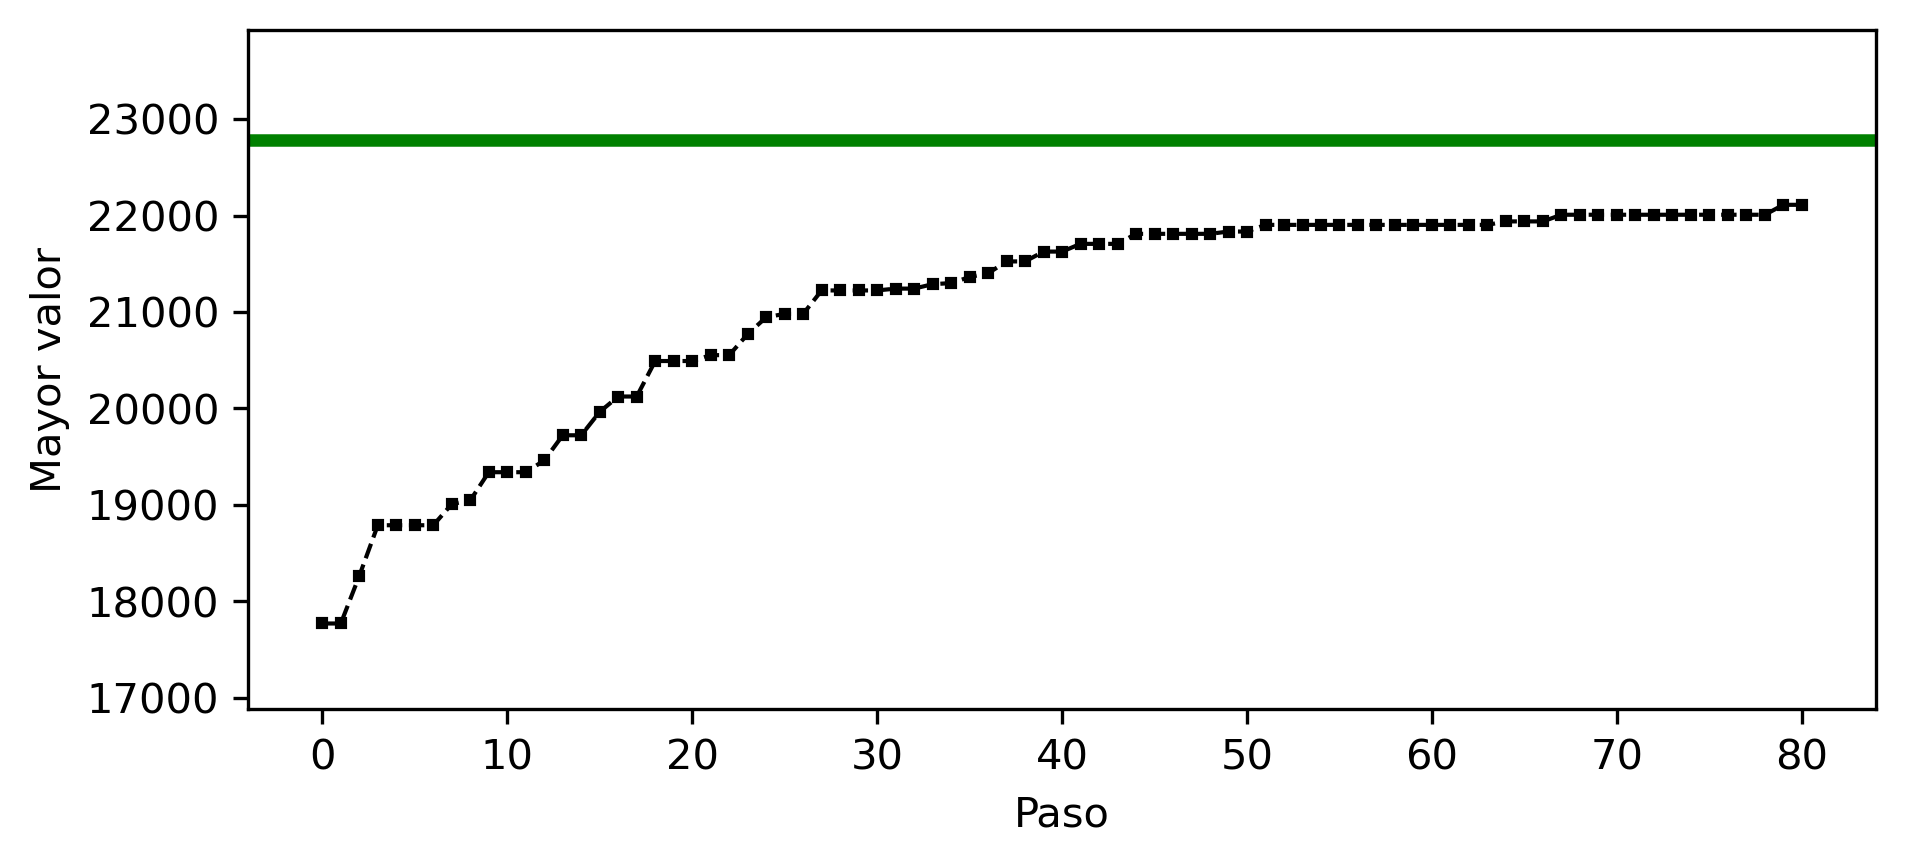
\includegraphics[width=\linewidth]{p10e_Prim_100.png}
\caption{Gráfica de primera instancia sin ruleta a 100 objetivos.}
\end{subfigure}
\begin{subfigure}[b]{0.40\linewidth}
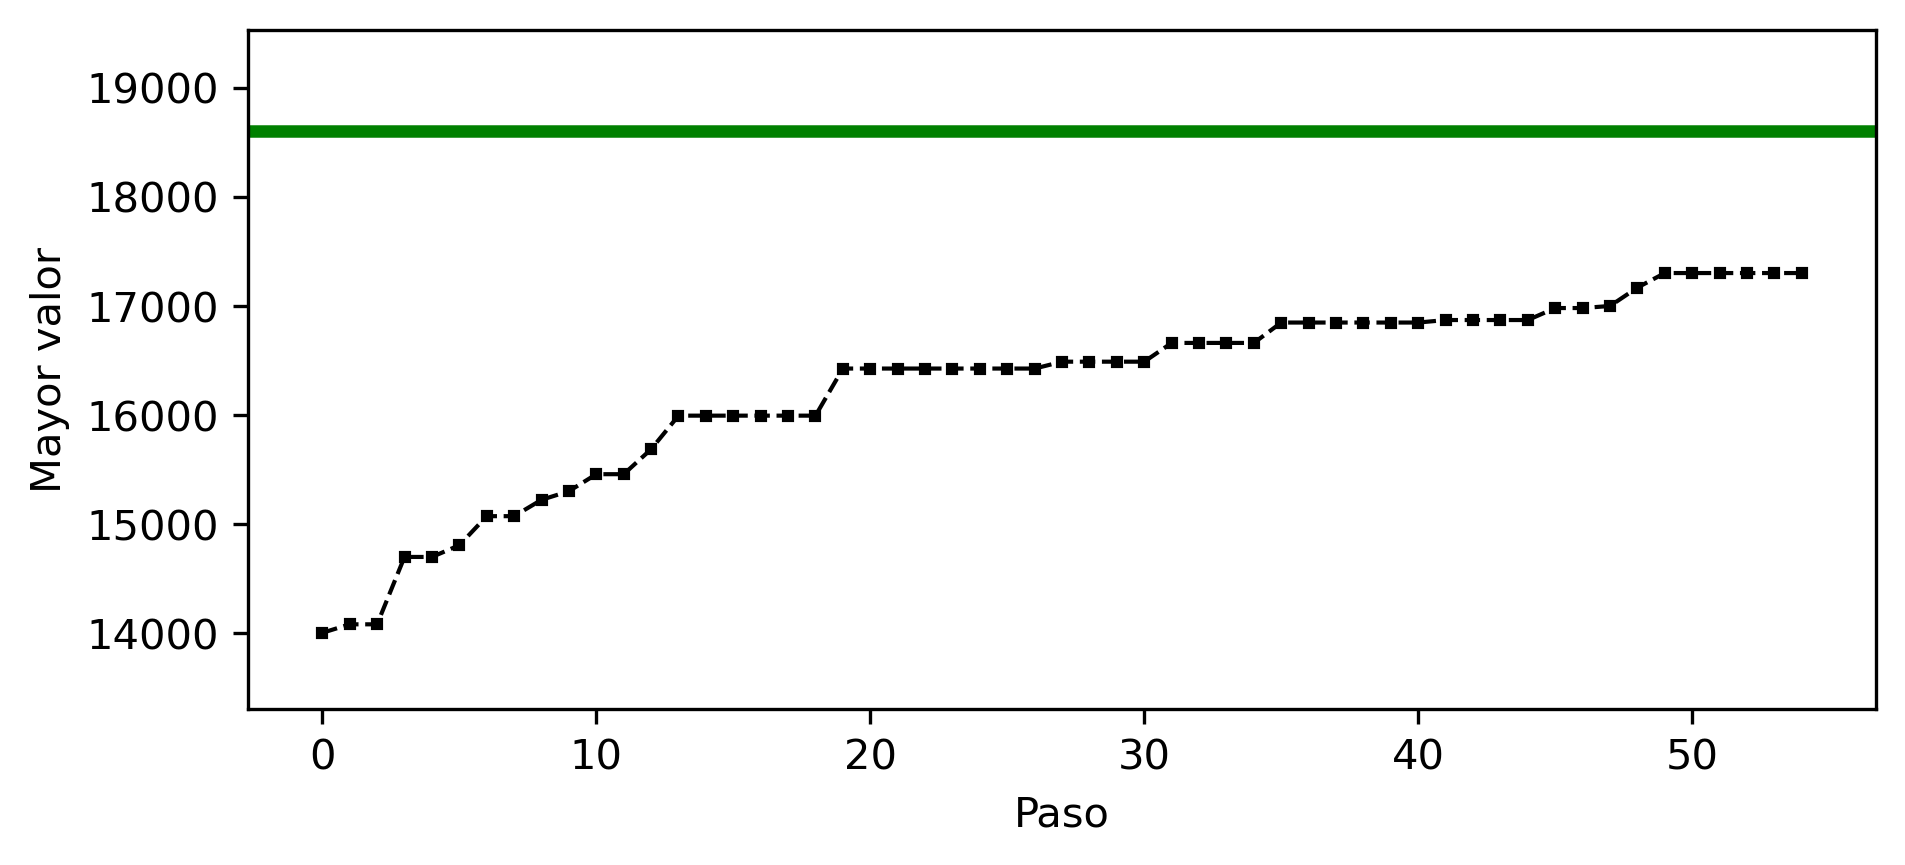
\includegraphics[width=\linewidth]{p10e_R_Prim_100.png}
\caption{Gráfica de primera instancia con ruleta a 100 objetivos.}
\end{subfigure}
\caption{Gráficas comparando el mayor valor.}
\label{fig:westminster}
\end{figure}

\begin{figure}[H]
\centering
\begin{subfigure}[b]{0.40\linewidth}
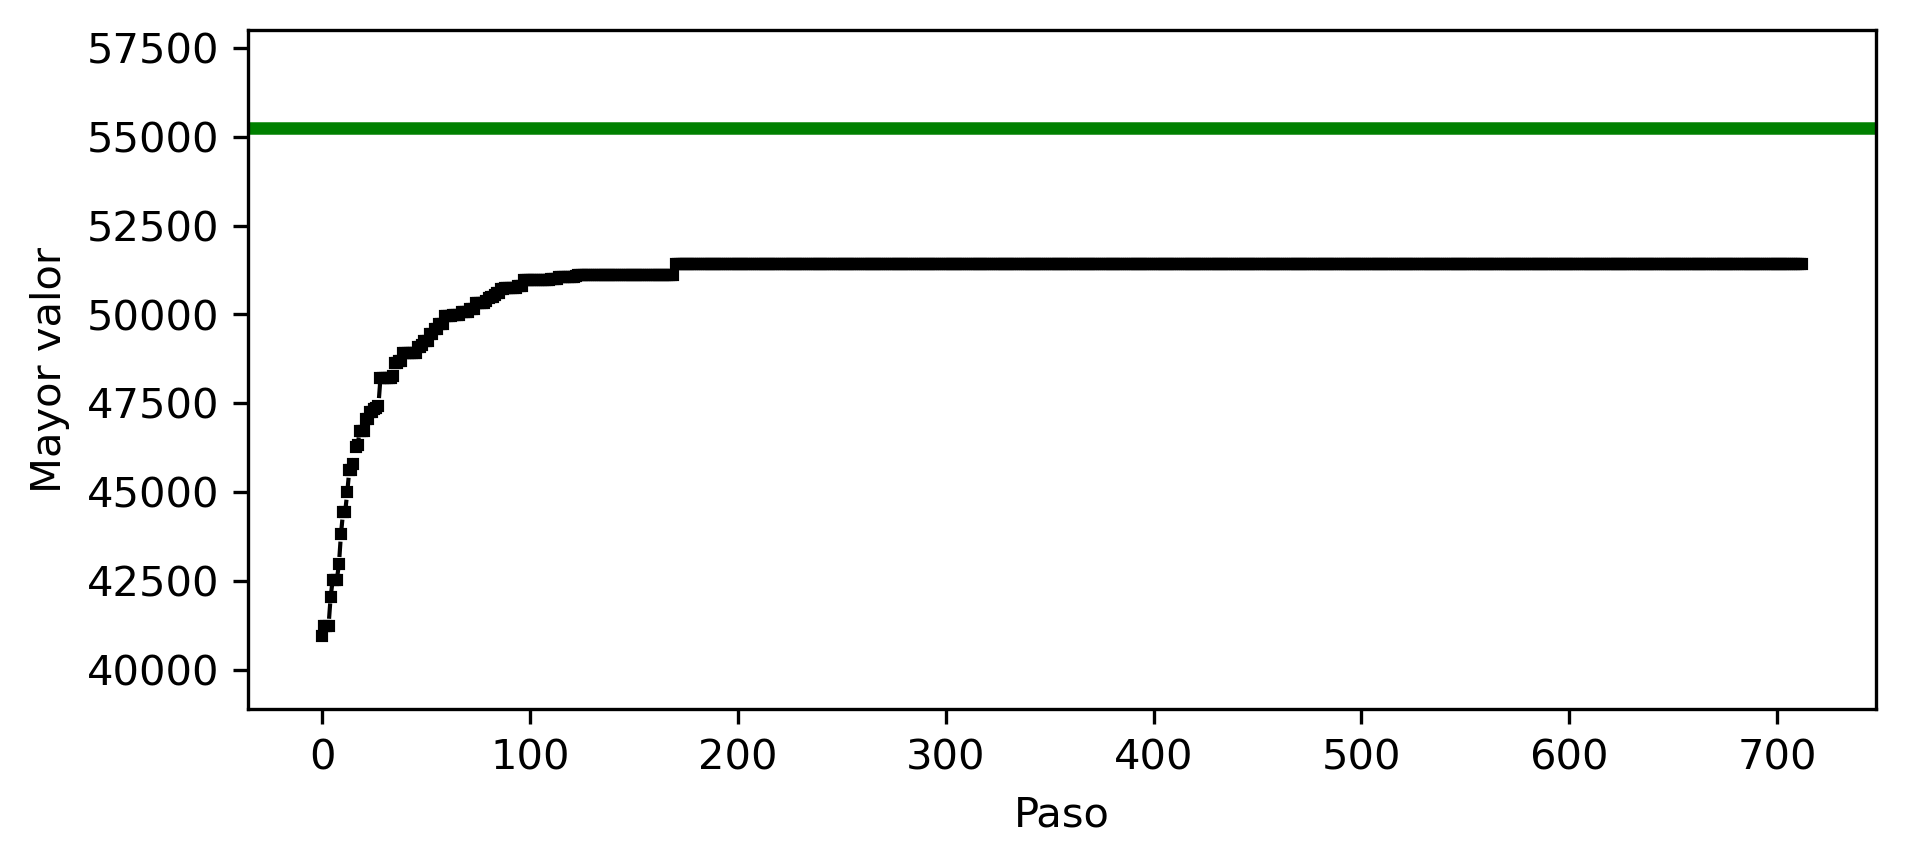
\includegraphics[width=\linewidth]{p10e_Prim_300.png}
\caption{Gráfica de primera instancia sin ruleta a 300 objetivos.}
\end{subfigure}
\begin{subfigure}[b]{0.40\linewidth}
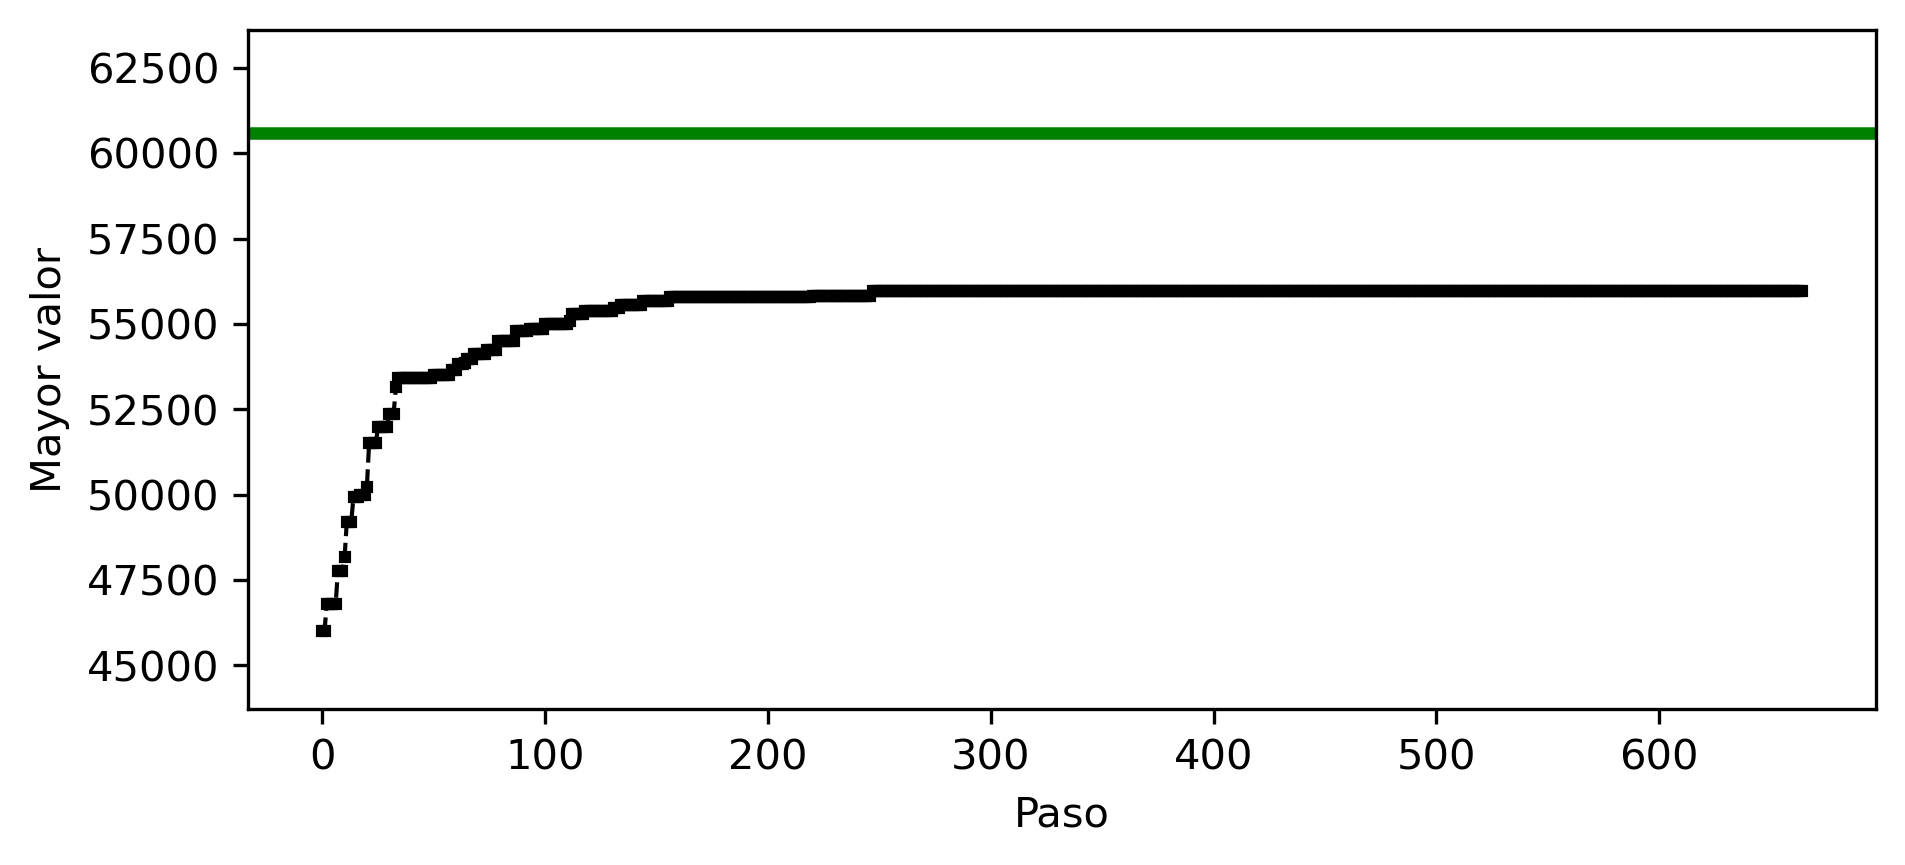
\includegraphics[width=\linewidth]{p10e_R_Prim_300.png}
\caption{Gráfica de primera instancia con ruleta a 300 objetivos.}
\end{subfigure}
\caption{Gráficas comparando el mayor valor.}
\label{fig:westminster}
\end{figure}

\begin{figure}[H]
\centering
\begin{subfigure}[b]{0.40\linewidth}
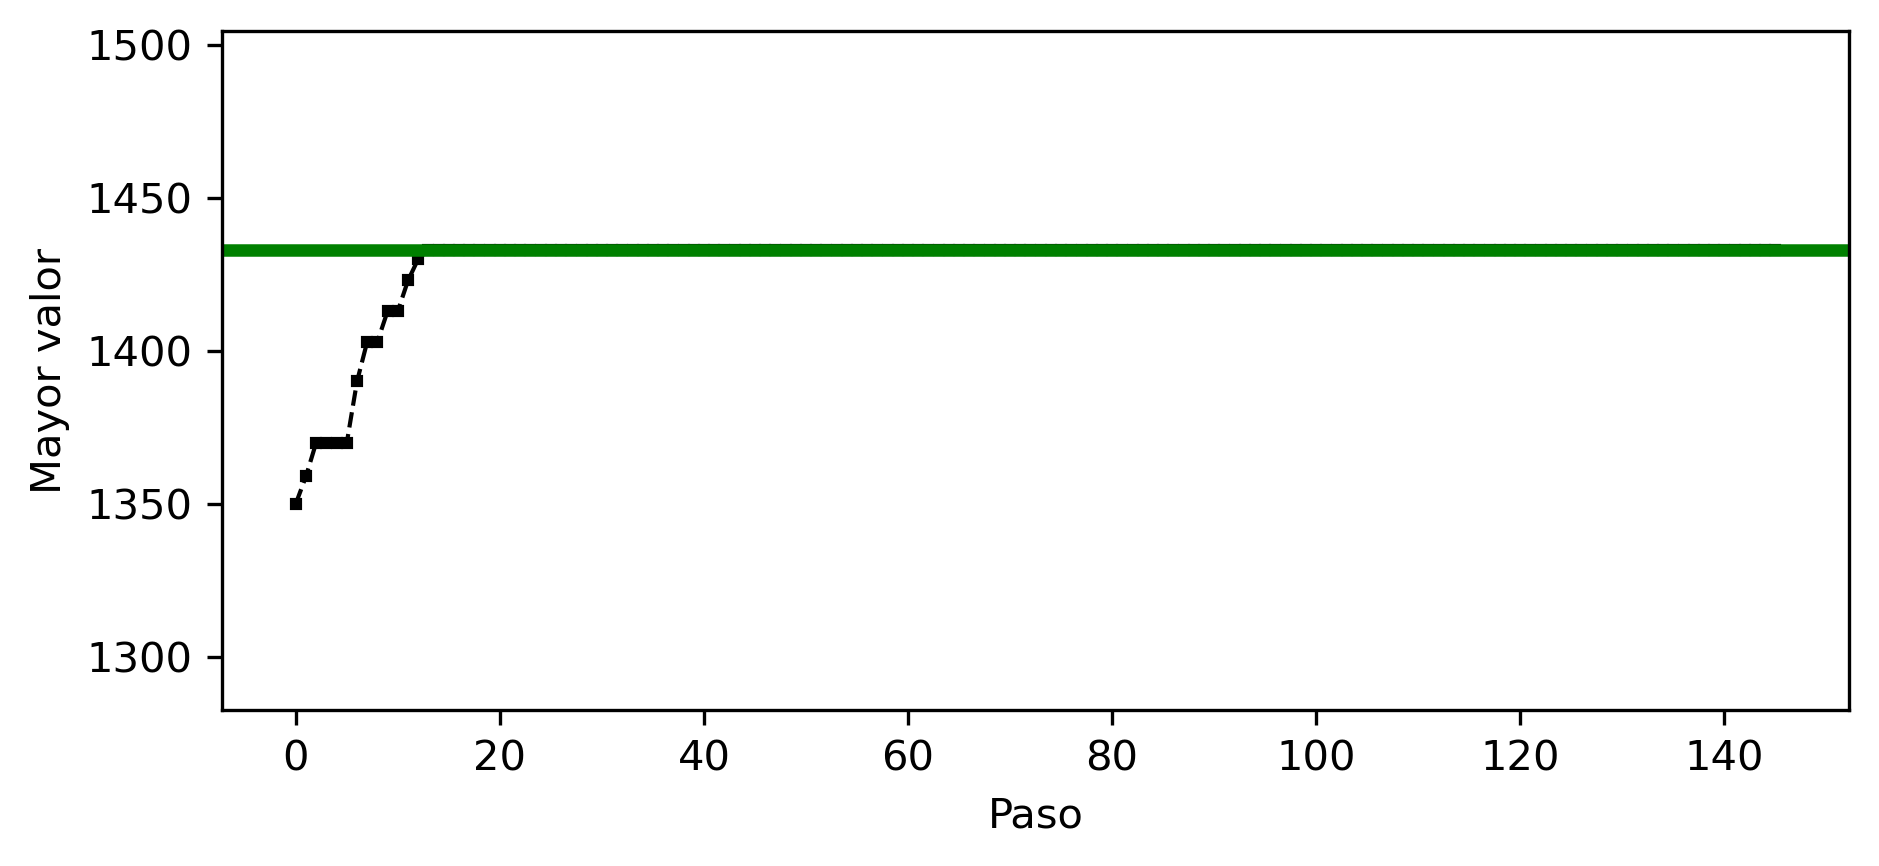
\includegraphics[width=\linewidth]{p10e_Seg_100.png}
\caption{Gráfica de segunda instancia sin ruleta a 100 objetivos.}
\end{subfigure}
\begin{subfigure}[b]{0.40\linewidth}
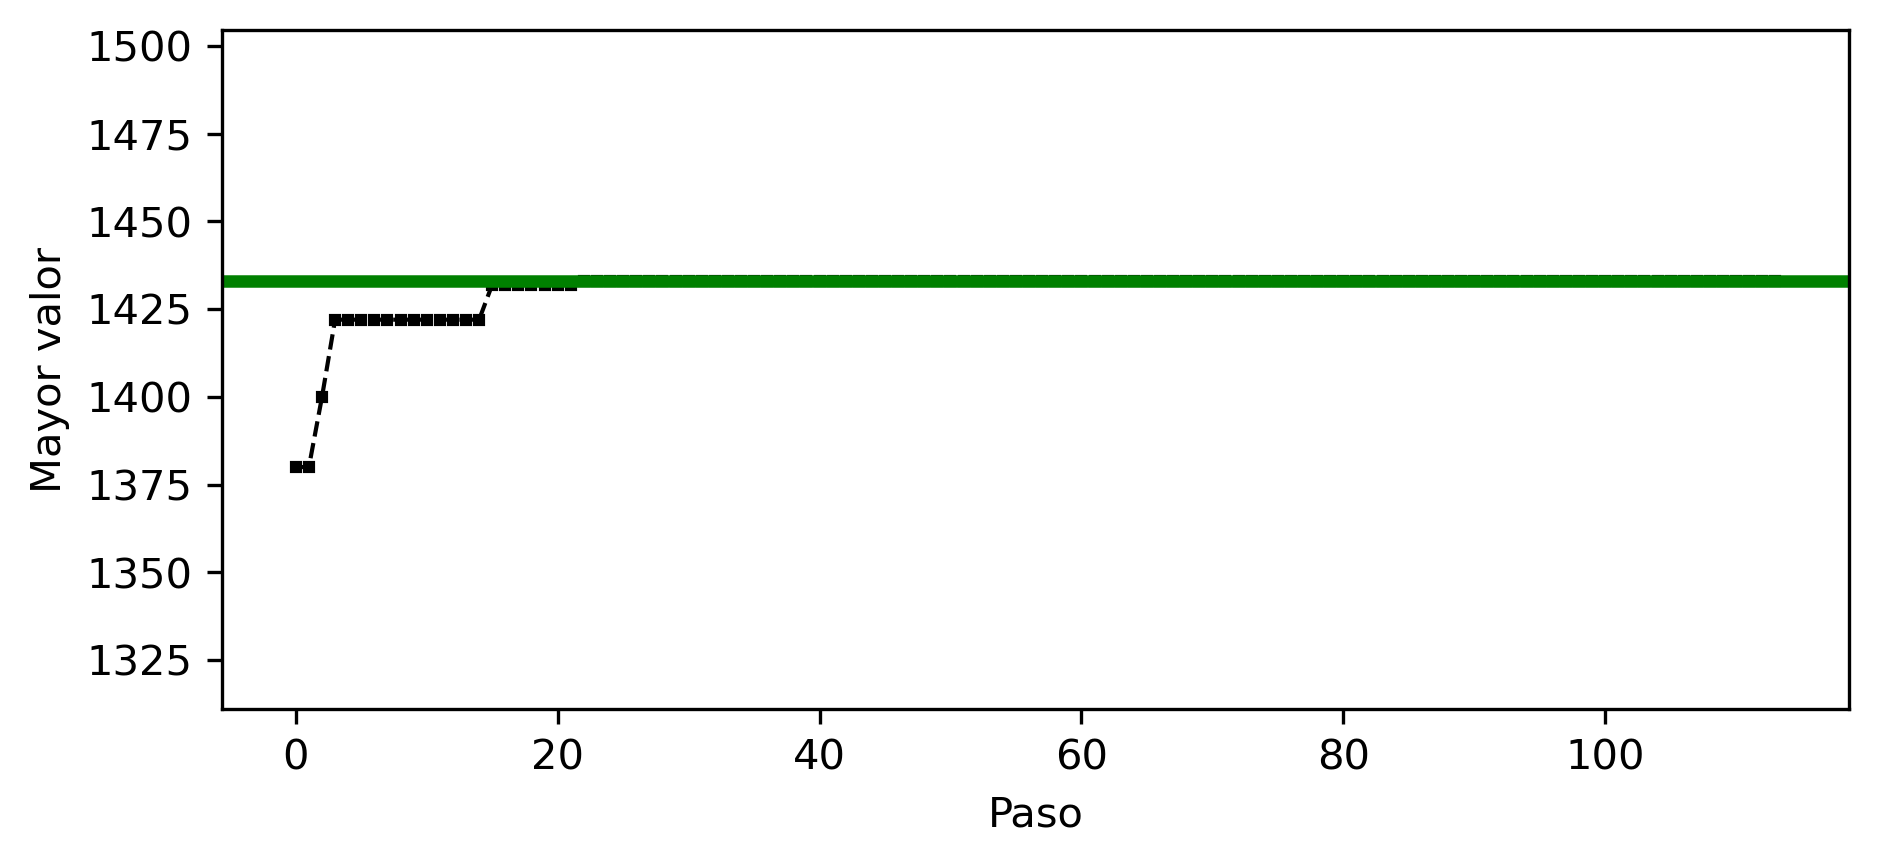
\includegraphics[width=\linewidth]{p10e_R_Seg_100.png}
\caption{Gráfica de primera instancia con ruleta a 100 objetivos.}
\end{subfigure}
\caption{Gráficas comparando el mayor valor.}
\label{fig:westminster}
\end{figure}

\begin{figure}[H]
\centering
\begin{subfigure}[b]{0.40\linewidth}
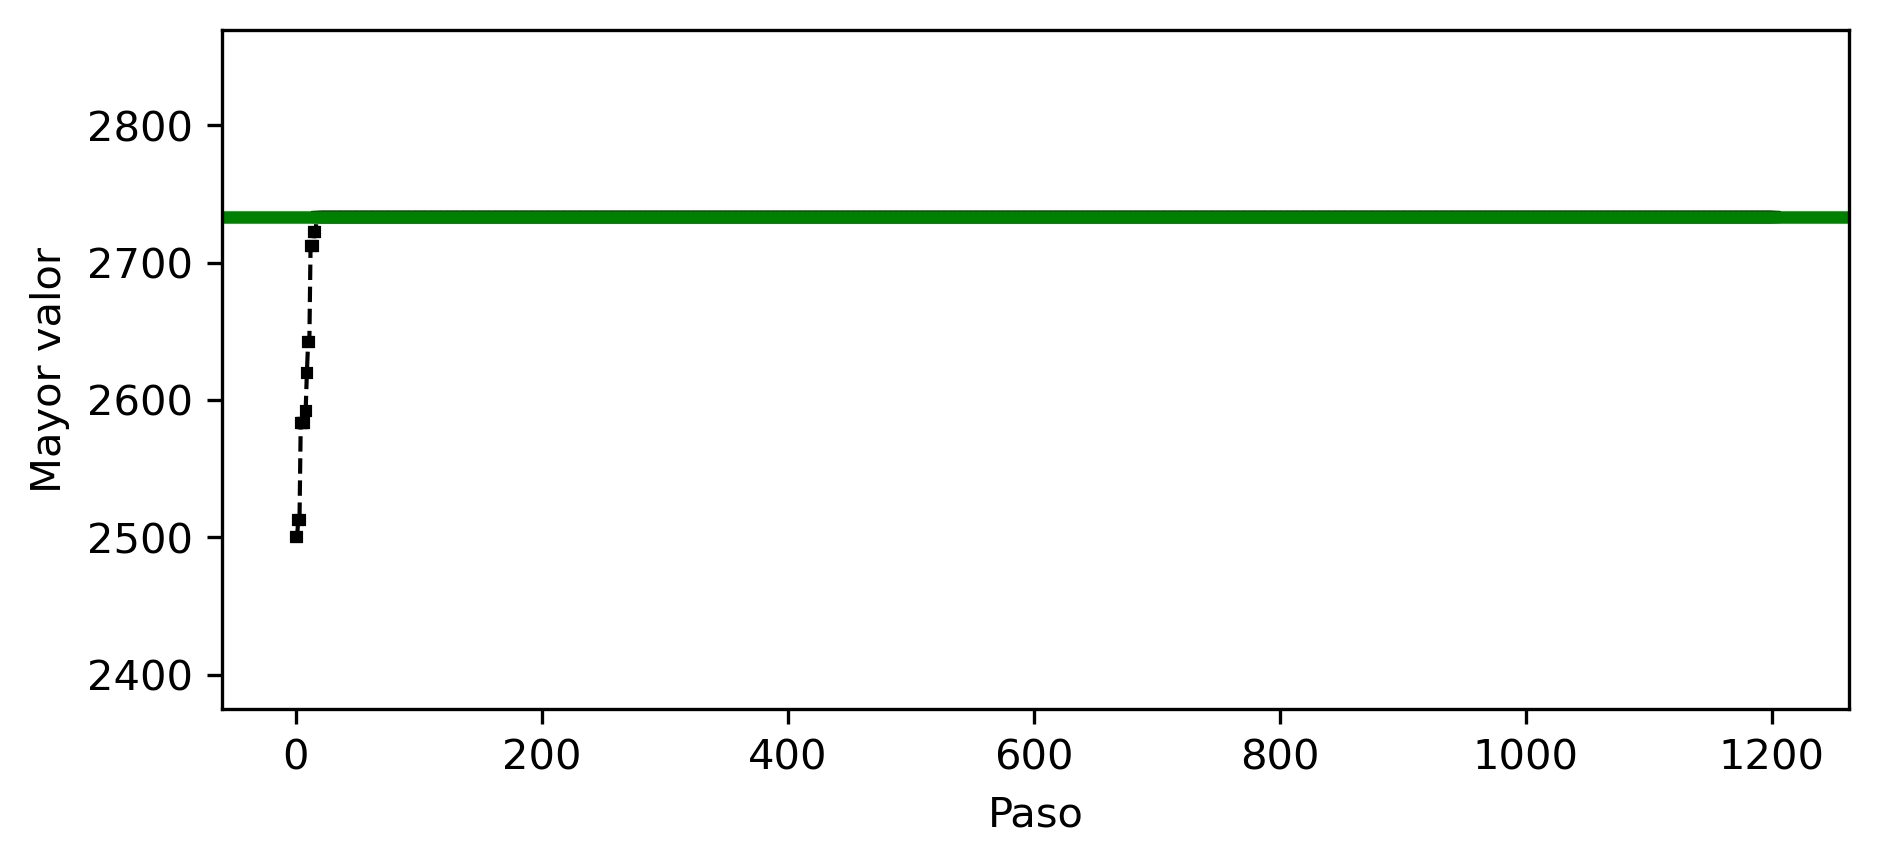
\includegraphics[width=\linewidth]{p10e_Seg_300.png}
\caption{Gráfica de segunda instancia sin ruleta a 300 objetivos.}
\end{subfigure}
\begin{subfigure}[b]{0.40\linewidth}
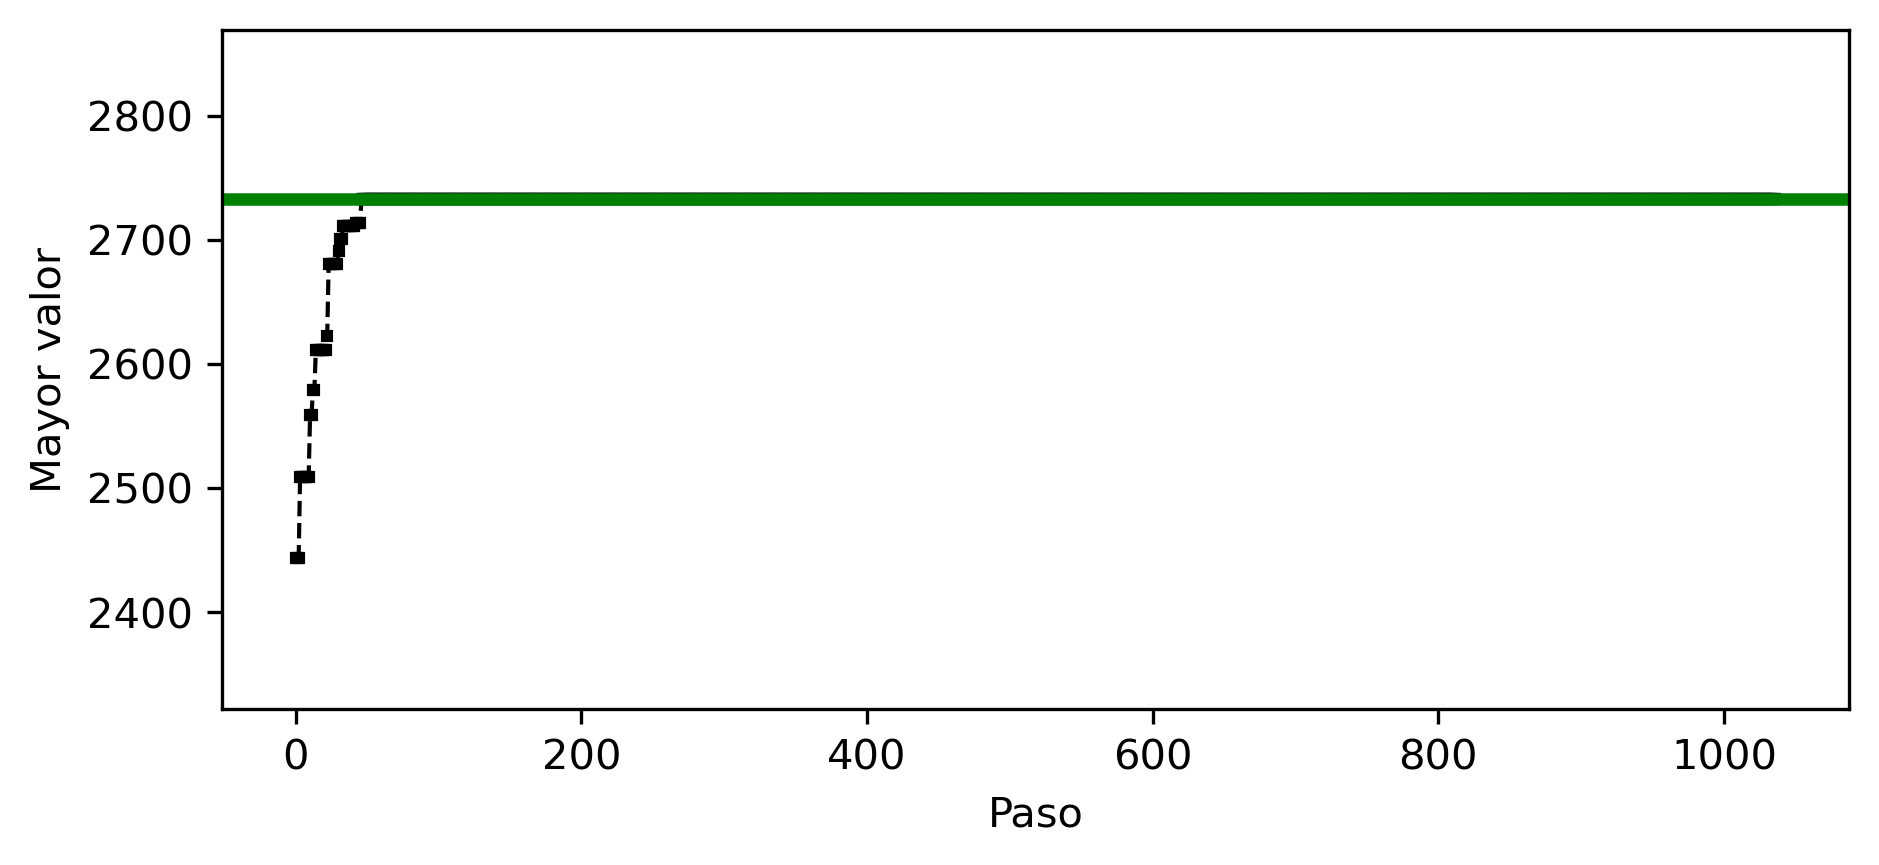
\includegraphics[width=\linewidth]{p10e_R_Seg_300.png}
\caption{Gráfica de segunda instancia con ruleta a 300 objetivoss.}
\end{subfigure}
\caption{Gráficas comparando el mayor valor.}
\label{fig:westminster}
\end{figure}

\begin{figure}[H]
\centering
\begin{subfigure}[b]{0.40\linewidth}
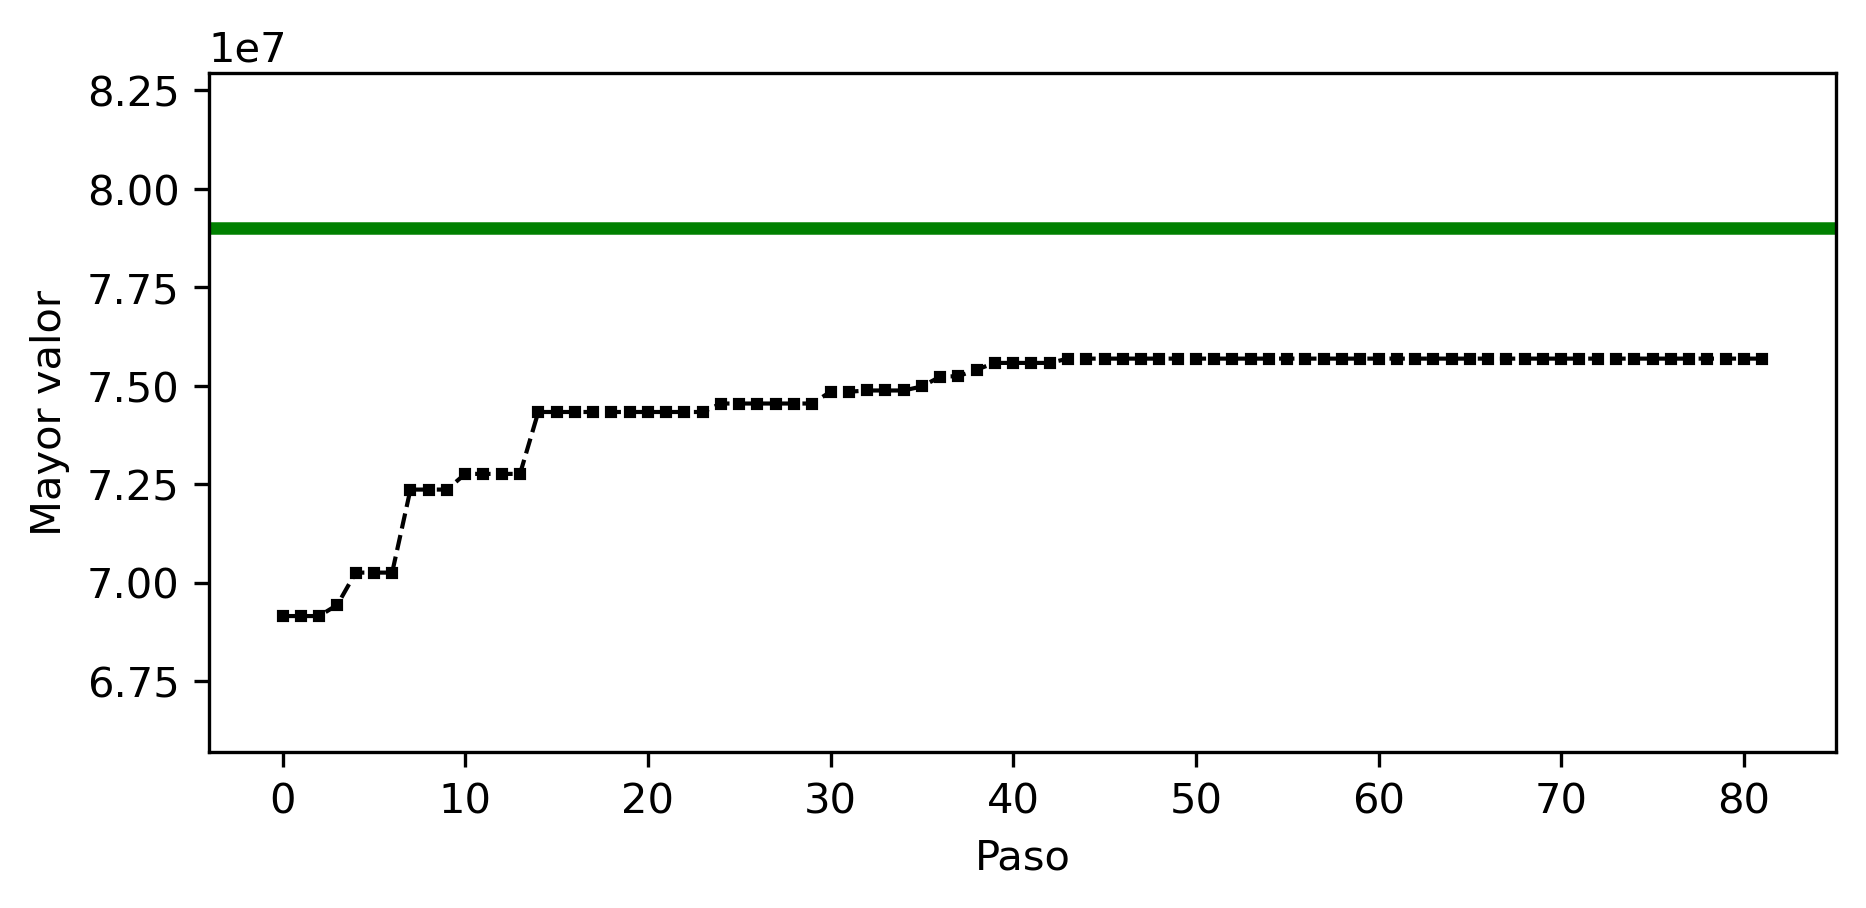
\includegraphics[width=\linewidth]{p10e_Ter_100.png}
\caption{Gráfica de tercer instancia sin ruleta a 100 objetivos.}
\end{subfigure}
\begin{subfigure}[b]{0.40\linewidth}
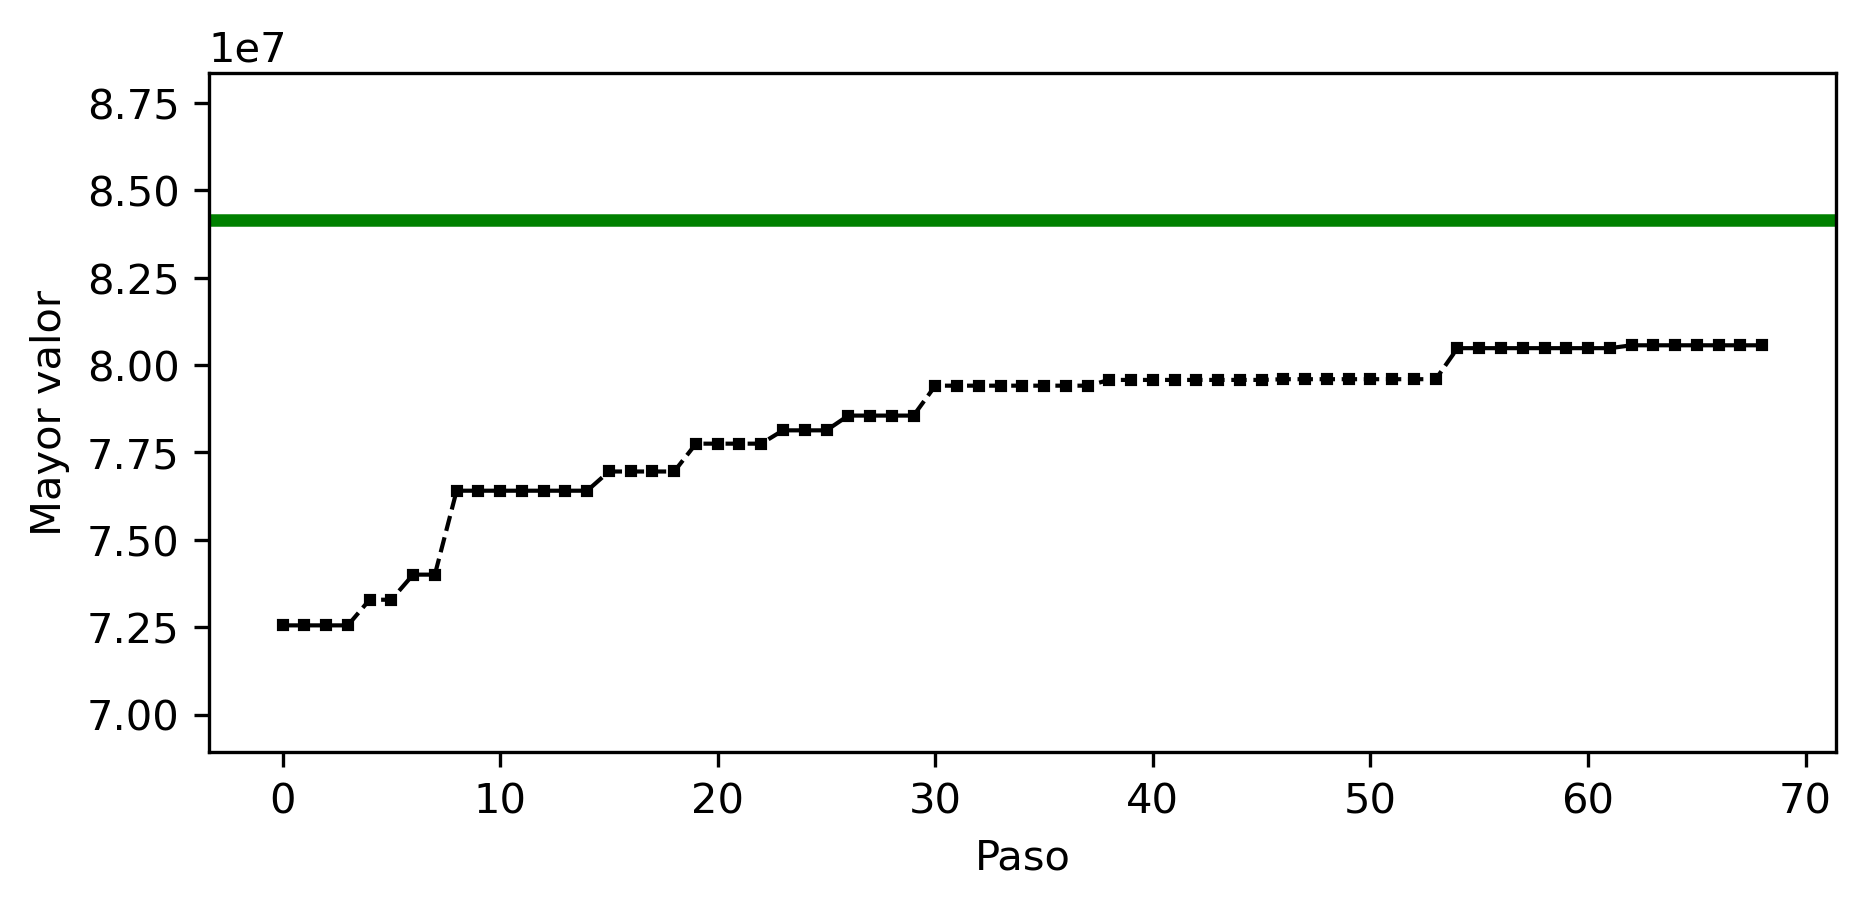
\includegraphics[width=\linewidth]{p10e_R_Ter_100.png}
\caption{Gráfica de tercer instancia con ruleta a 100 objetivos.}
\end{subfigure}
\caption{Gráficas comparando el mayor valor.}
\label{fig:westminster}
\end{figure}

\begin{figure}[H]
\centering
\begin{subfigure}[b]{0.40\linewidth}
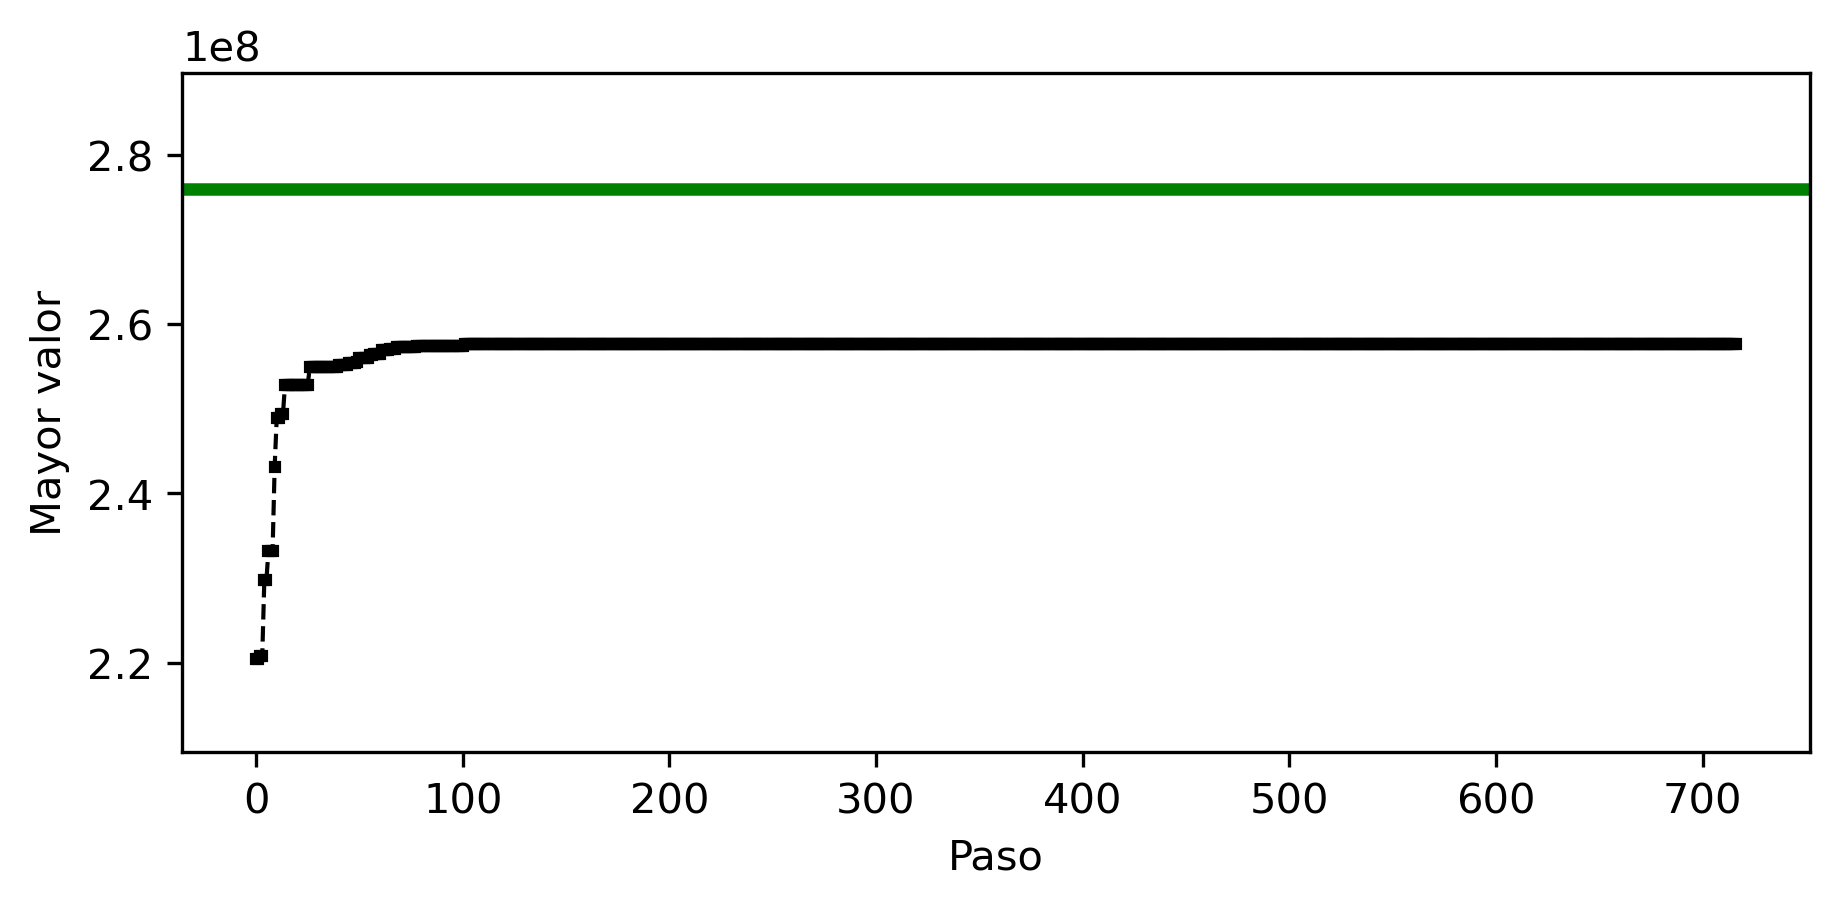
\includegraphics[width=\linewidth]{p10e_Ter_300.png}
\caption{Gráfica de tercer instancia sin ruleta a 300 objetivos.}
\end{subfigure}
\begin{subfigure}[b]{0.40\linewidth}
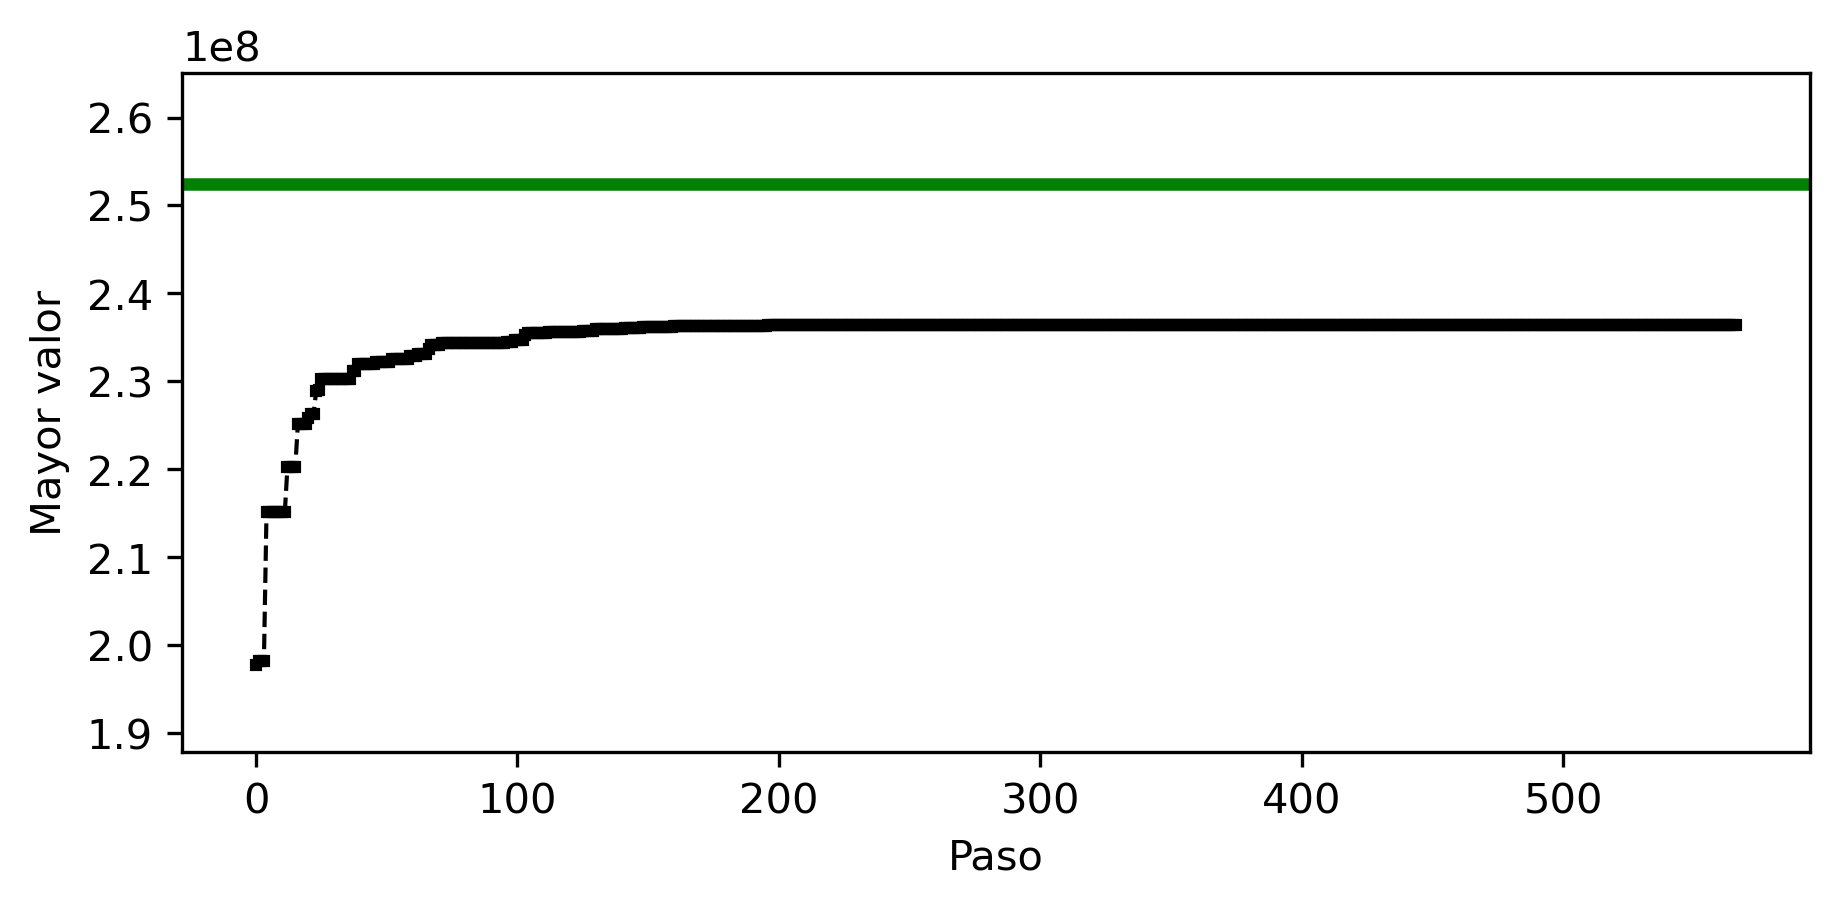
\includegraphics[width=\linewidth]{p10e_R_Ter_300.png}
\caption{Gráfica de tercer instancia con ruleta a 300 objetivos.}
\end{subfigure}
\caption{Gráficas comparando el mayor valor.}
\label{fig:westminster}
\end{figure}

\begin{figure}[H]
\centering
\begin{subfigure}[b]{0.40\linewidth}
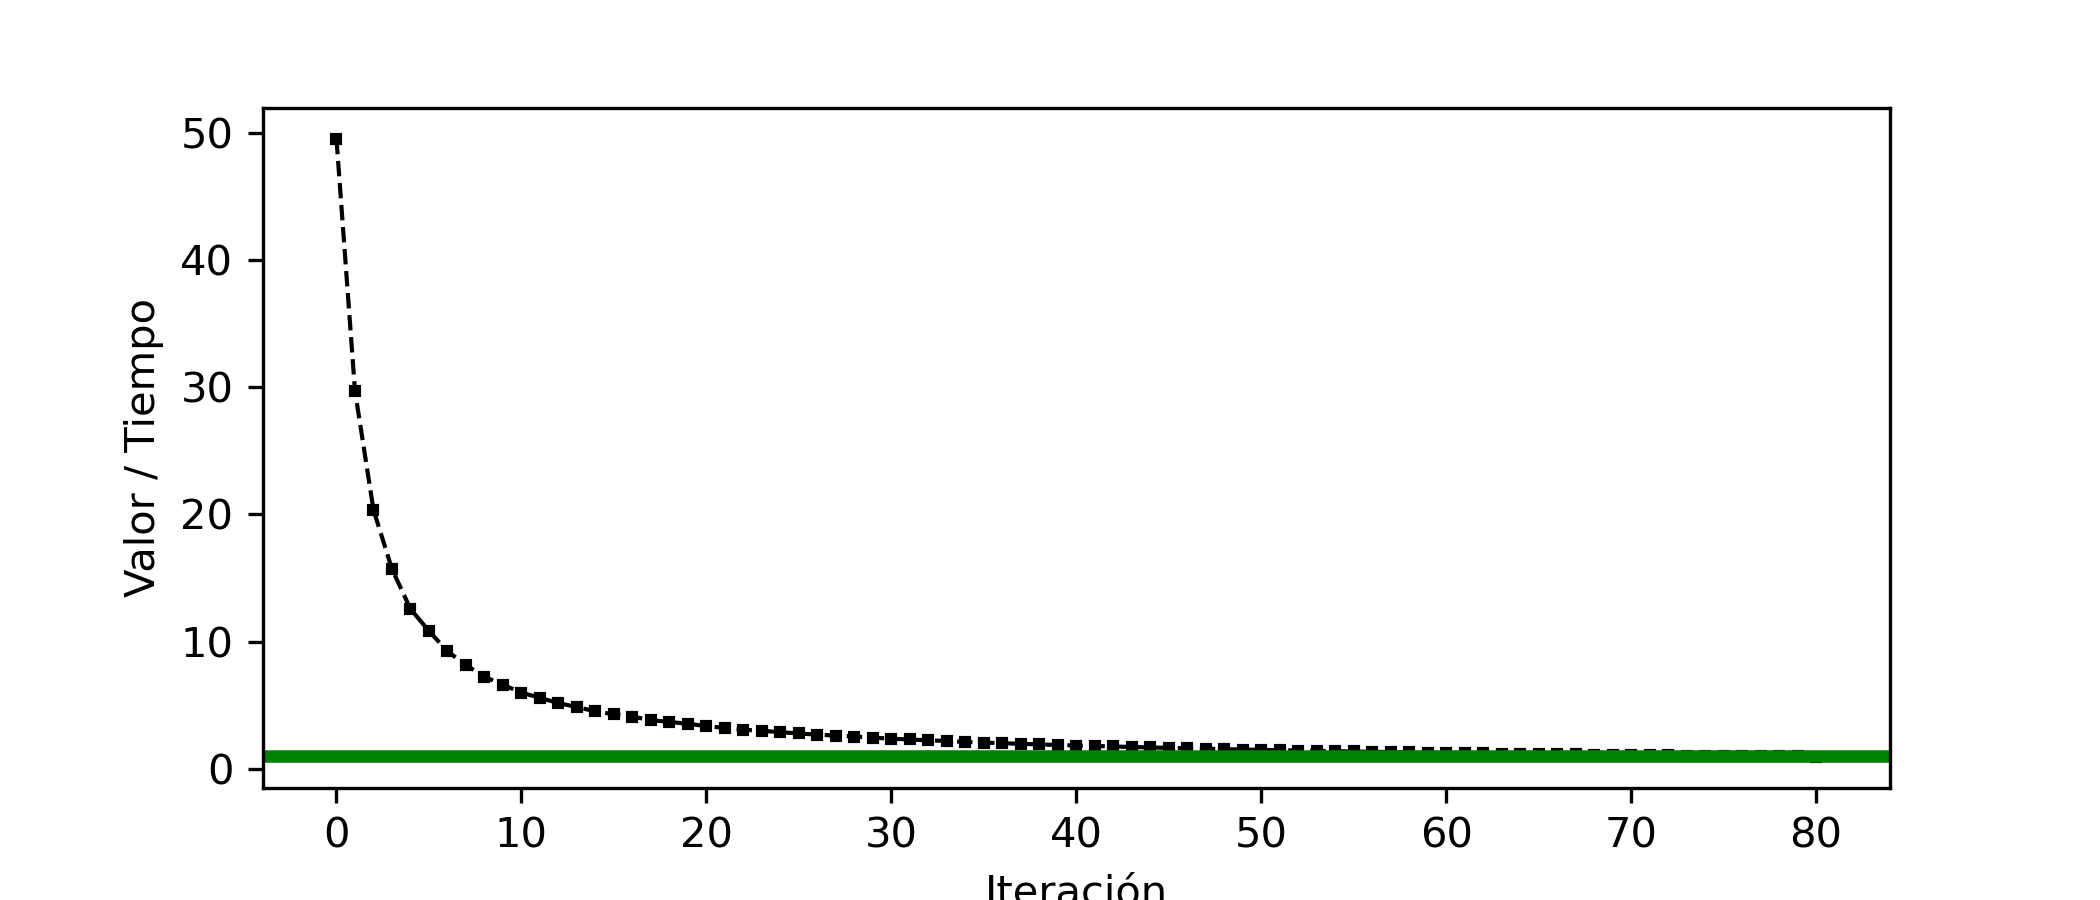
\includegraphics[width=\linewidth]{p10p_Prim_100.png}
\caption{Gráfica de primer instancia sin ruleta a 100 objetivos.}
\end{subfigure}
\begin{subfigure}[b]{0.40\linewidth}
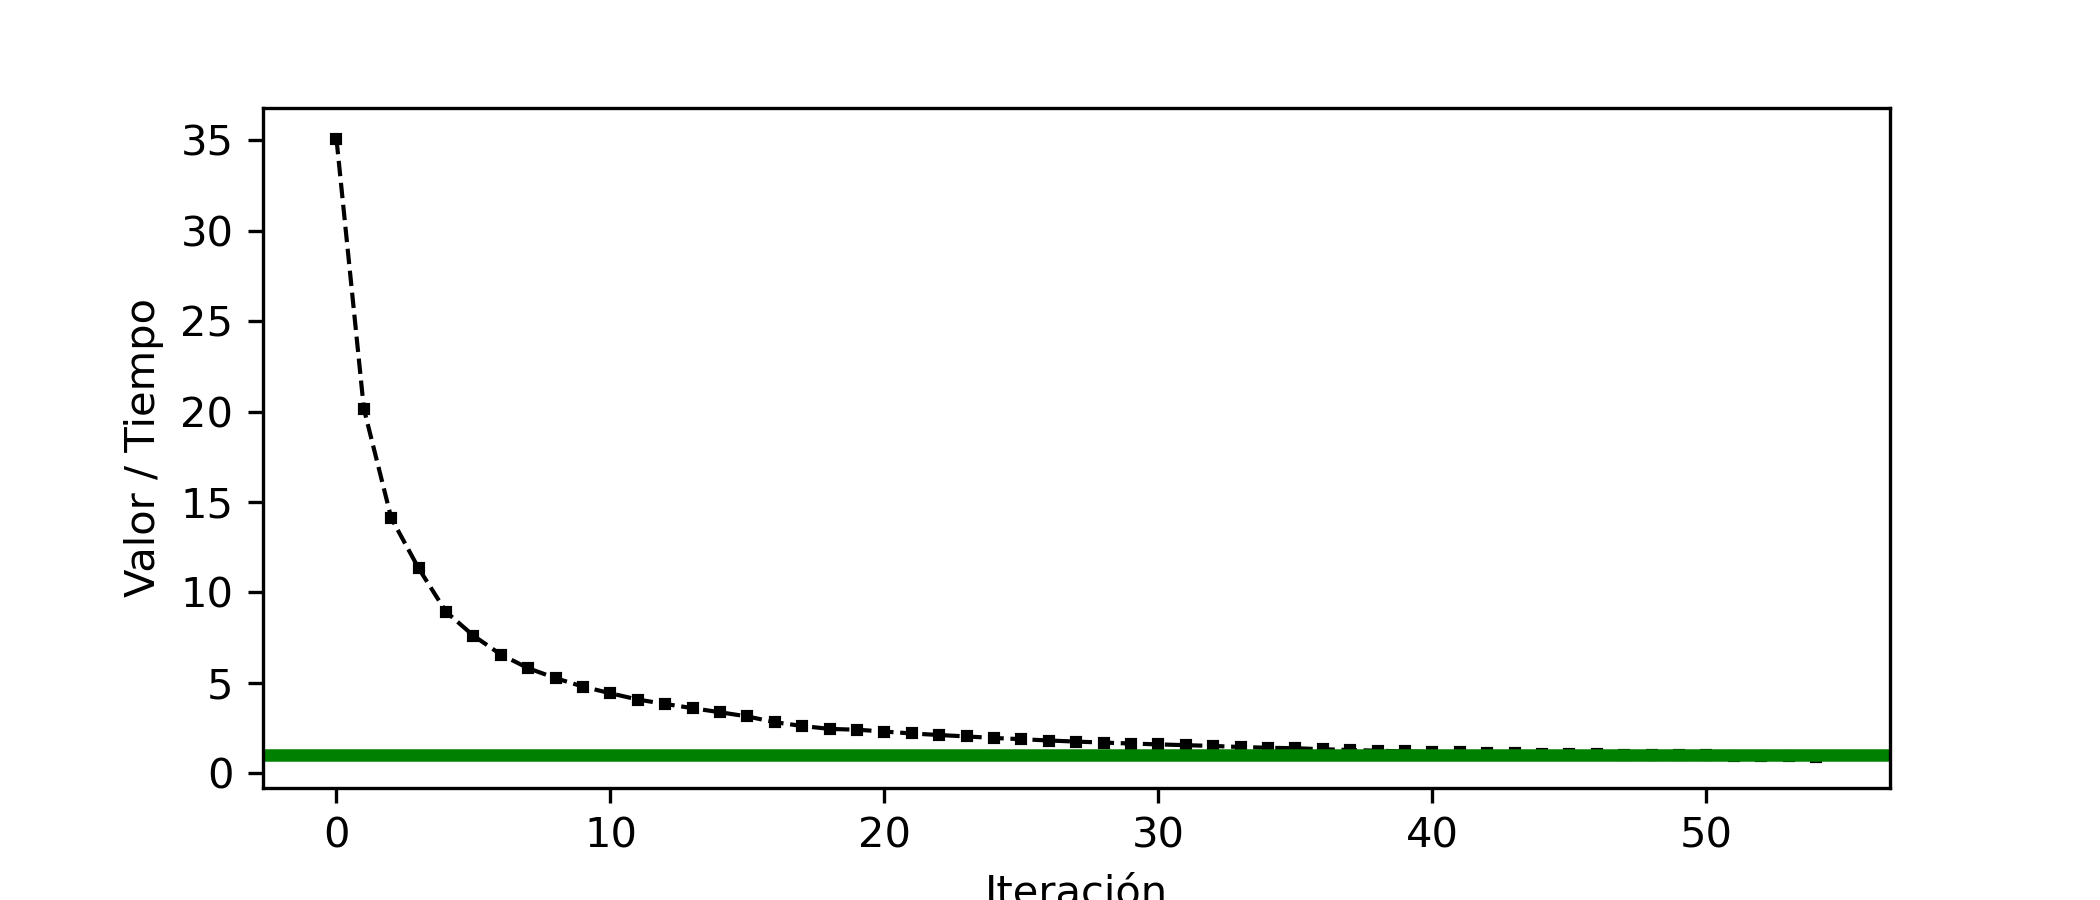
\includegraphics[width=\linewidth]{p10p_R_Prim_100.png}
\caption{Gráfica de primer instancia con ruleta a 100 objetivos.}
\end{subfigure}
\caption{Gráfica comparando valor sobre tiempo.}
\label{fig:westminster}
\end{figure}

\begin{figure}[H]
\centering
\begin{subfigure}[b]{0.40\linewidth}
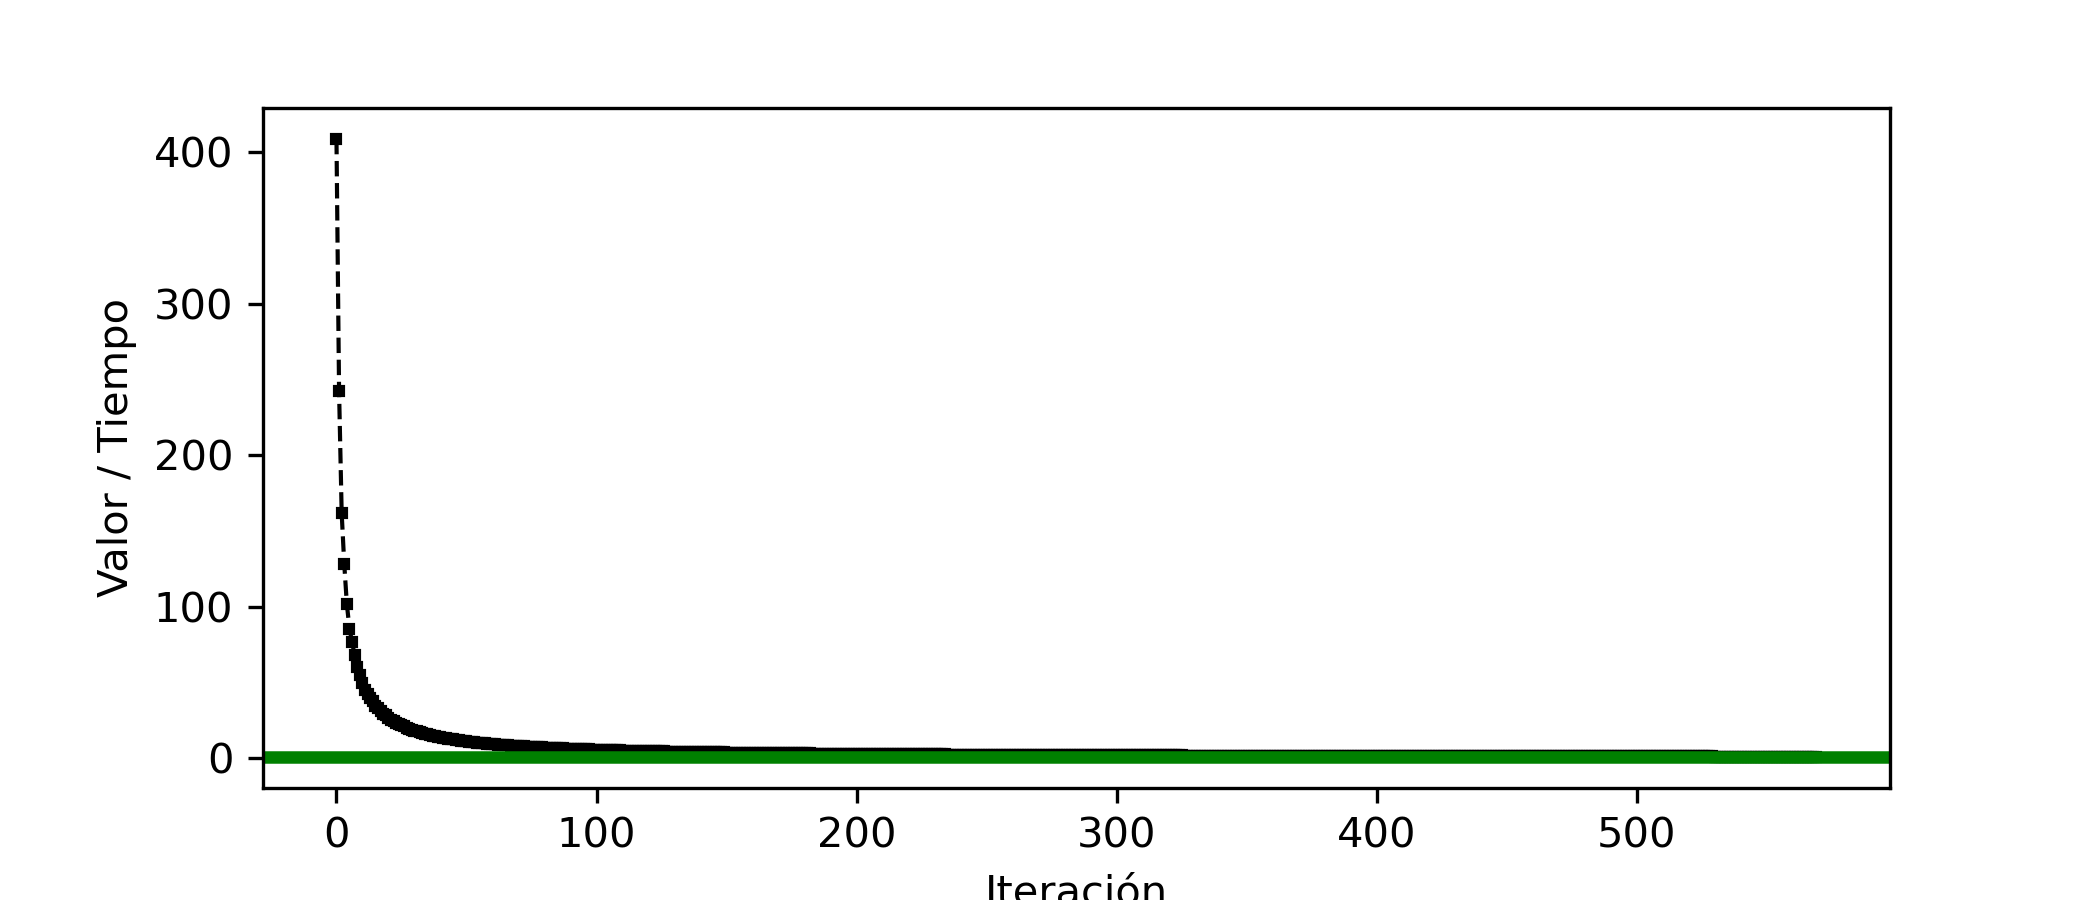
\includegraphics[width=\linewidth]{p10p_Seg_200.png}
\caption{Gráfica de segunda instancia sin ruleta a 200 objetivos.}
\end{subfigure}
\begin{subfigure}[b]{0.40\linewidth}
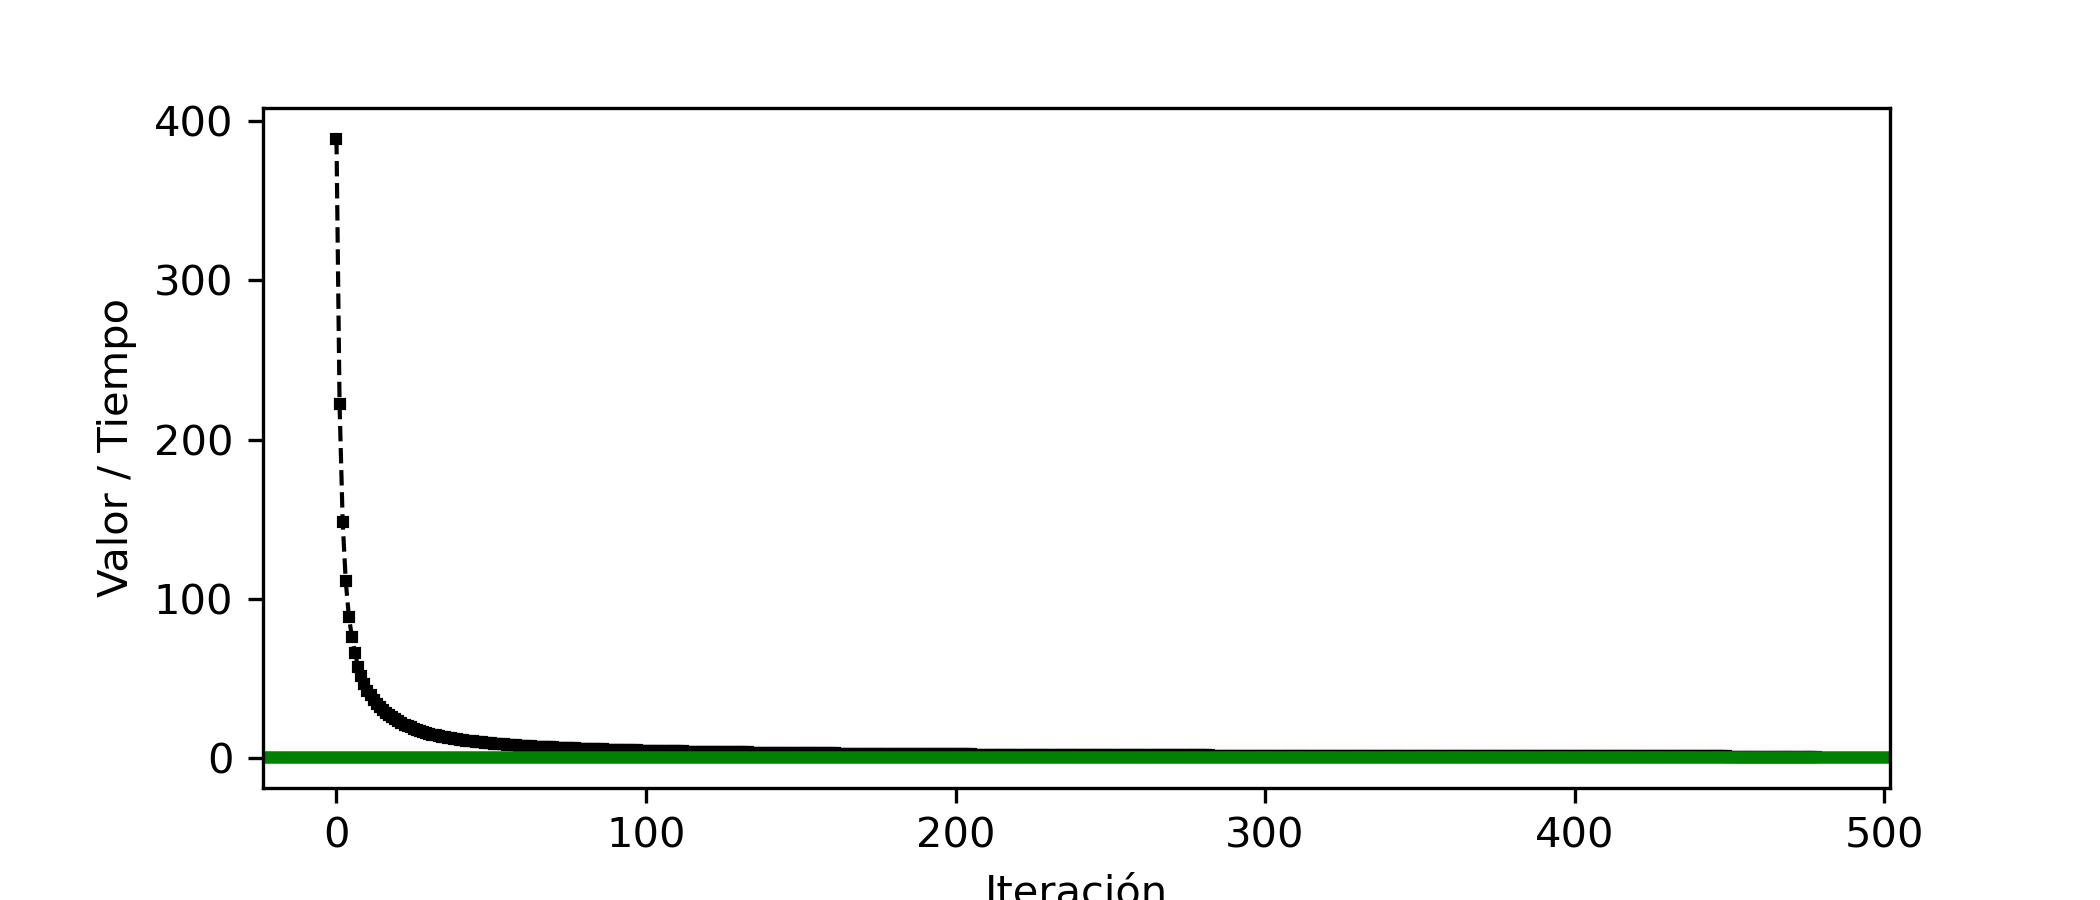
\includegraphics[width=\linewidth]{p10p_R_Seg_200.png}
\caption{Gráfica de segunda instancia con ruleta a 200 objetivos.}
\end{subfigure}
\caption{Gráfica comparando valor sobre tiempo.}
\label{fig:westminster}
\end{figure}

\begin{figure}[H]
\centering
\begin{subfigure}[b]{0.40\linewidth}
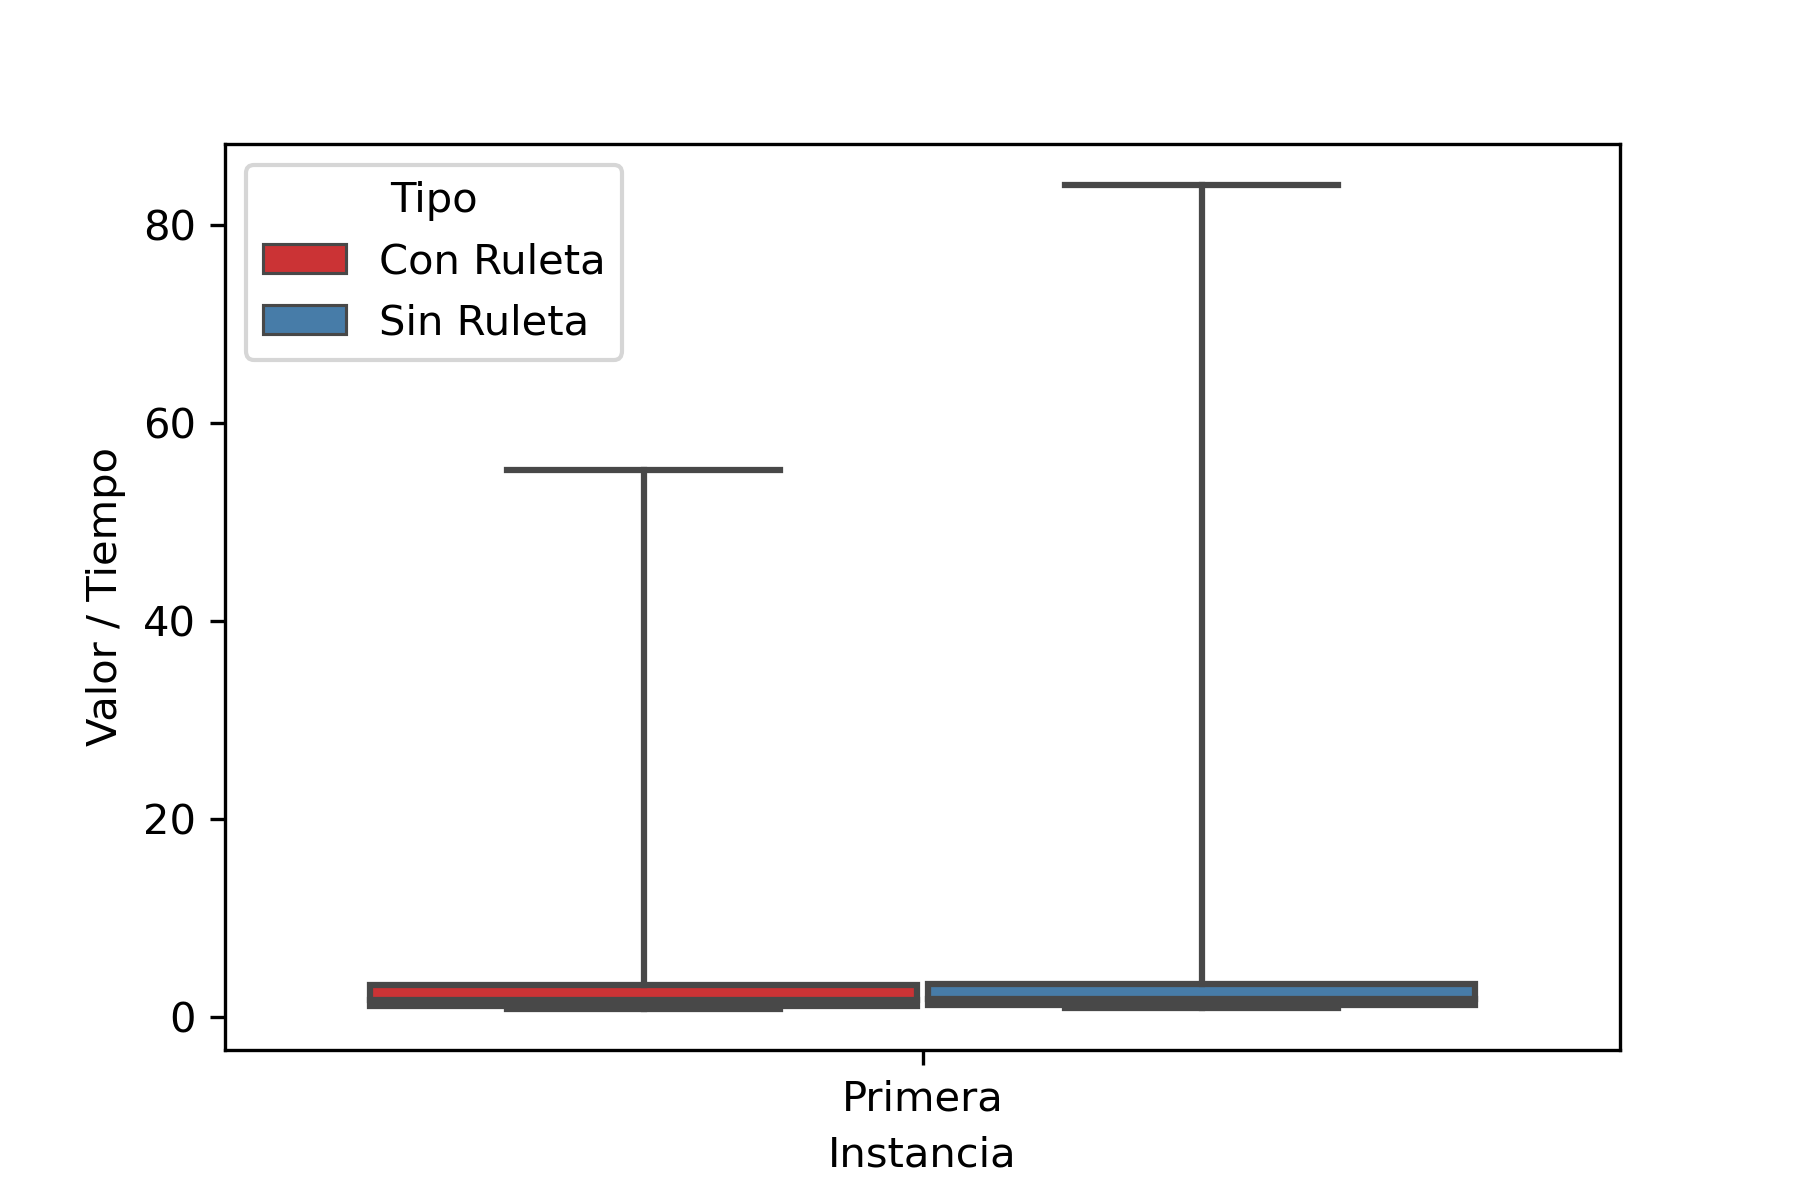
\includegraphics[width=\linewidth]{p10p_Box_Prim_100.png}
\caption{Caja bigote de primera instancia con 100 objetivos.}
\end{subfigure}
\begin{subfigure}[b]{0.40\linewidth}
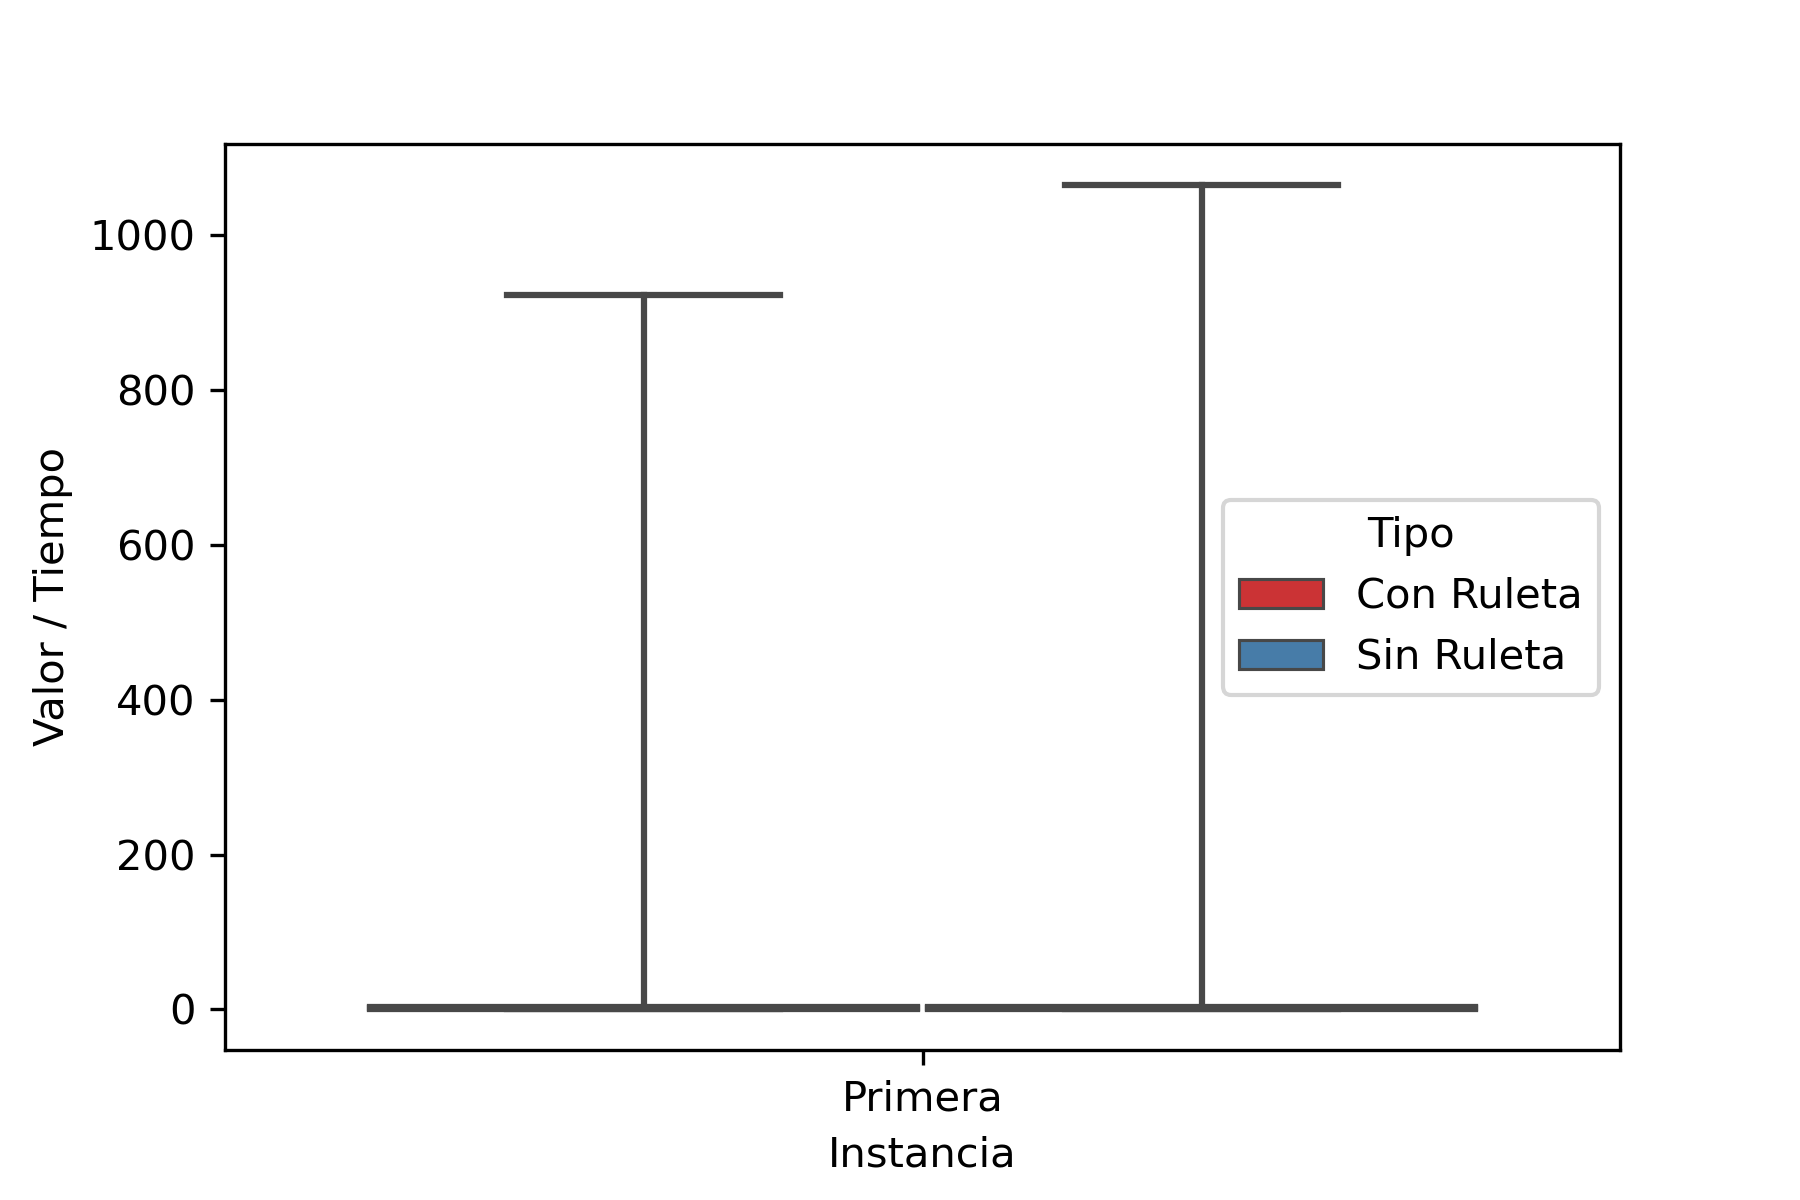
\includegraphics[width=\linewidth]{p10p_Box_Prim_400.png}
\caption{Caja bigote de primera instancia con 400 objetivos.}
\end{subfigure}
\caption{Caja bigote comparando valor sobre tiempo para cada instancia.}
\label{fig:westminster}
\end{figure}

\begin{figure}[H]
\centering
\begin{subfigure}[b]{0.40\linewidth}
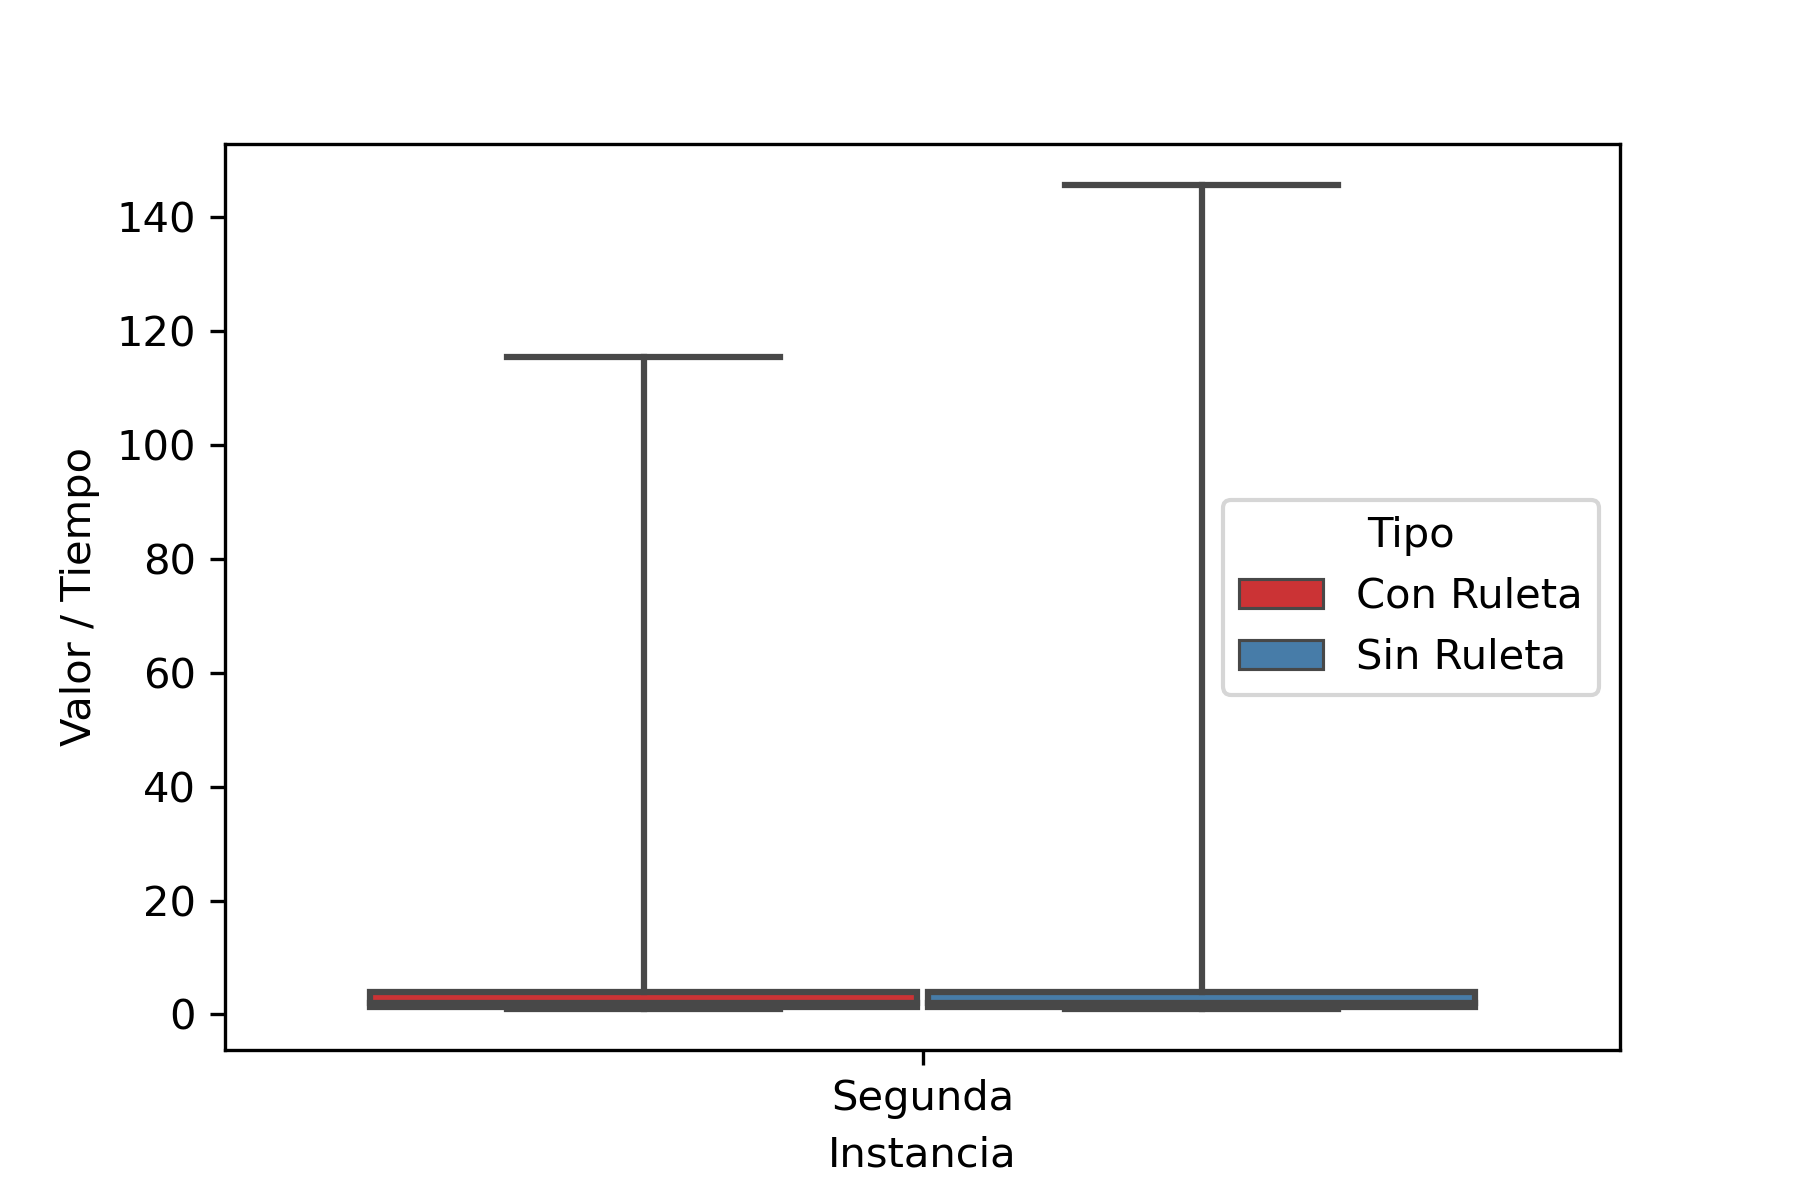
\includegraphics[width=\linewidth]{p10p_Box_Seg_100.png}
\caption{Caja bigote de segunda instancia con 100 objetivos.}
\end{subfigure}
\begin{subfigure}[b]{0.40\linewidth}
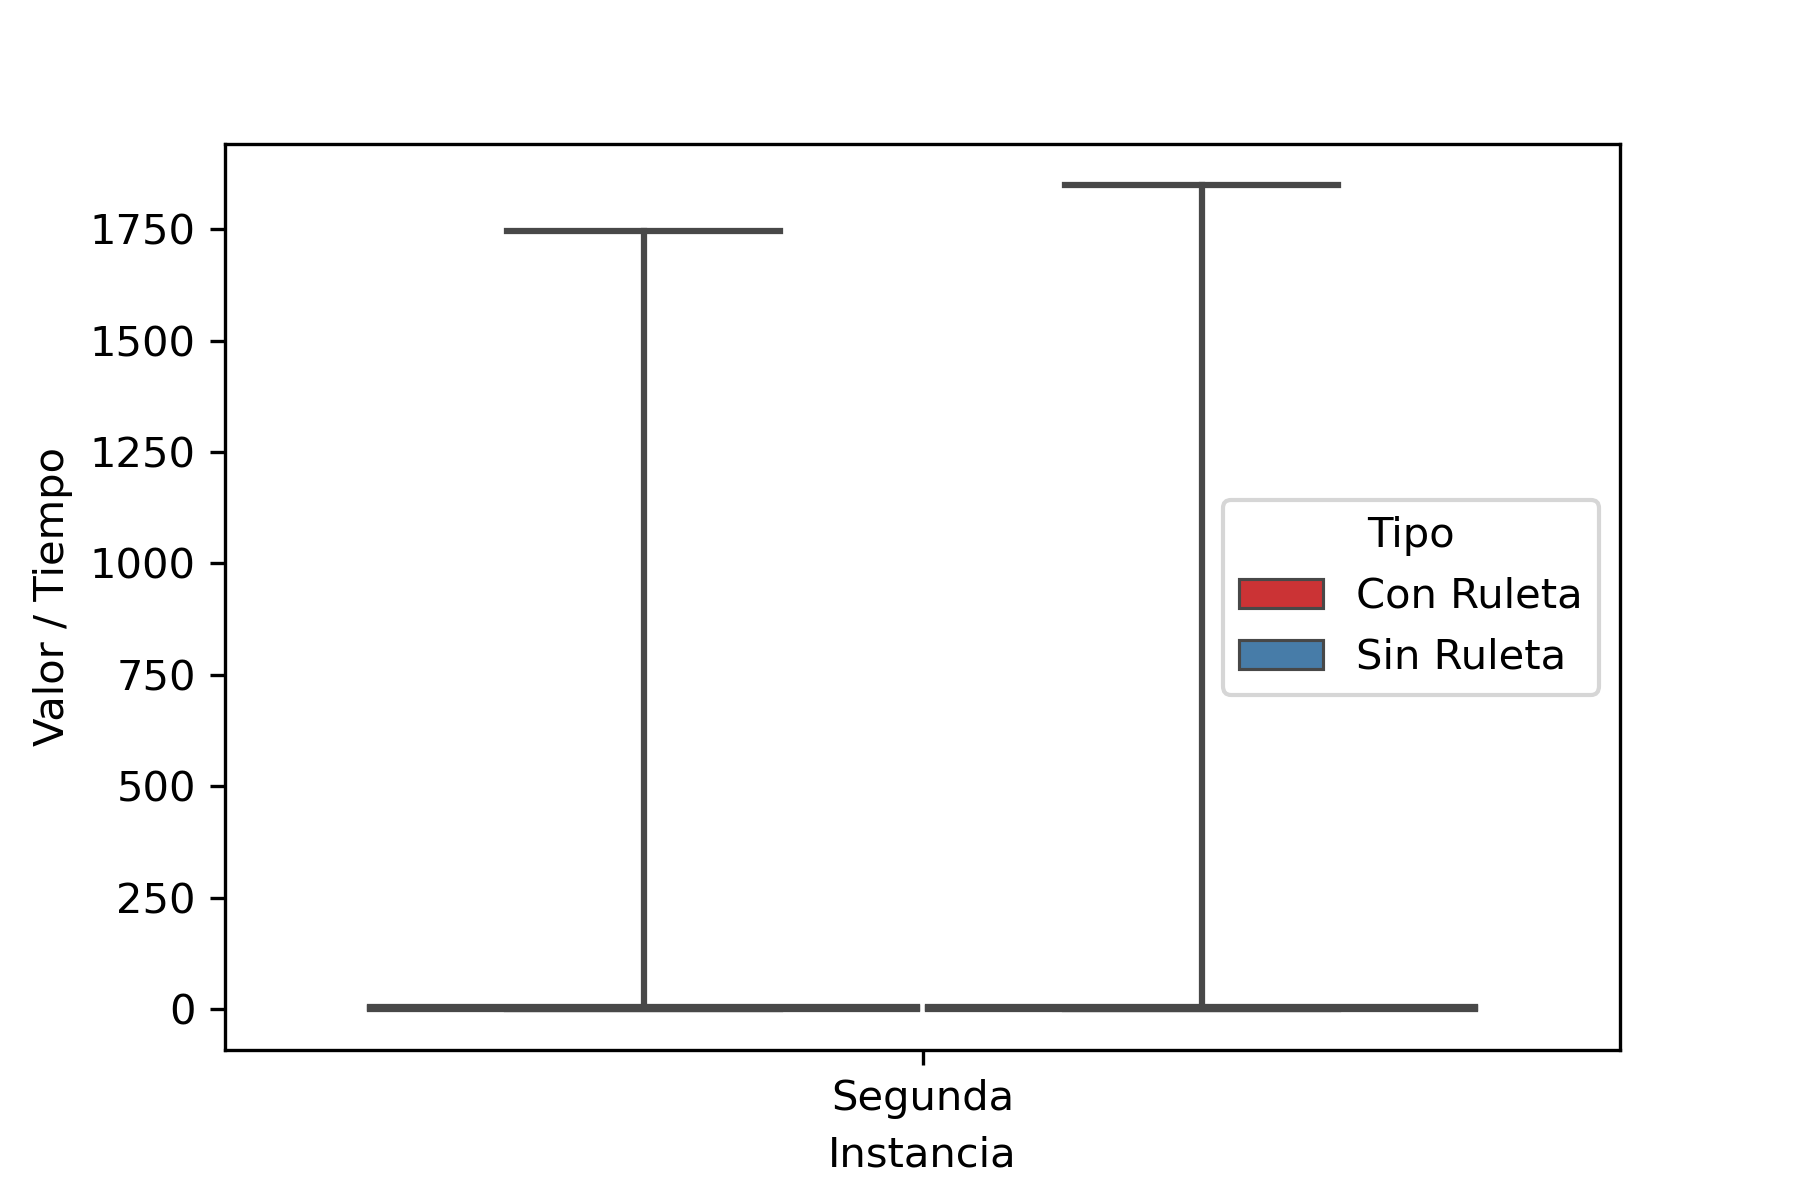
\includegraphics[width=\linewidth]{p10p_Box_Seg_400.png}
\caption{Caja bigote de segunda instancia con 400 objetivos.}
\end{subfigure}
\caption{Caja bigote comparando valor sobre tiempo para cada instancia.}
\label{fig:westminster}
\end{figure}

\begin{figure}[H]
\centering
\begin{subfigure}[b]{0.40\linewidth}
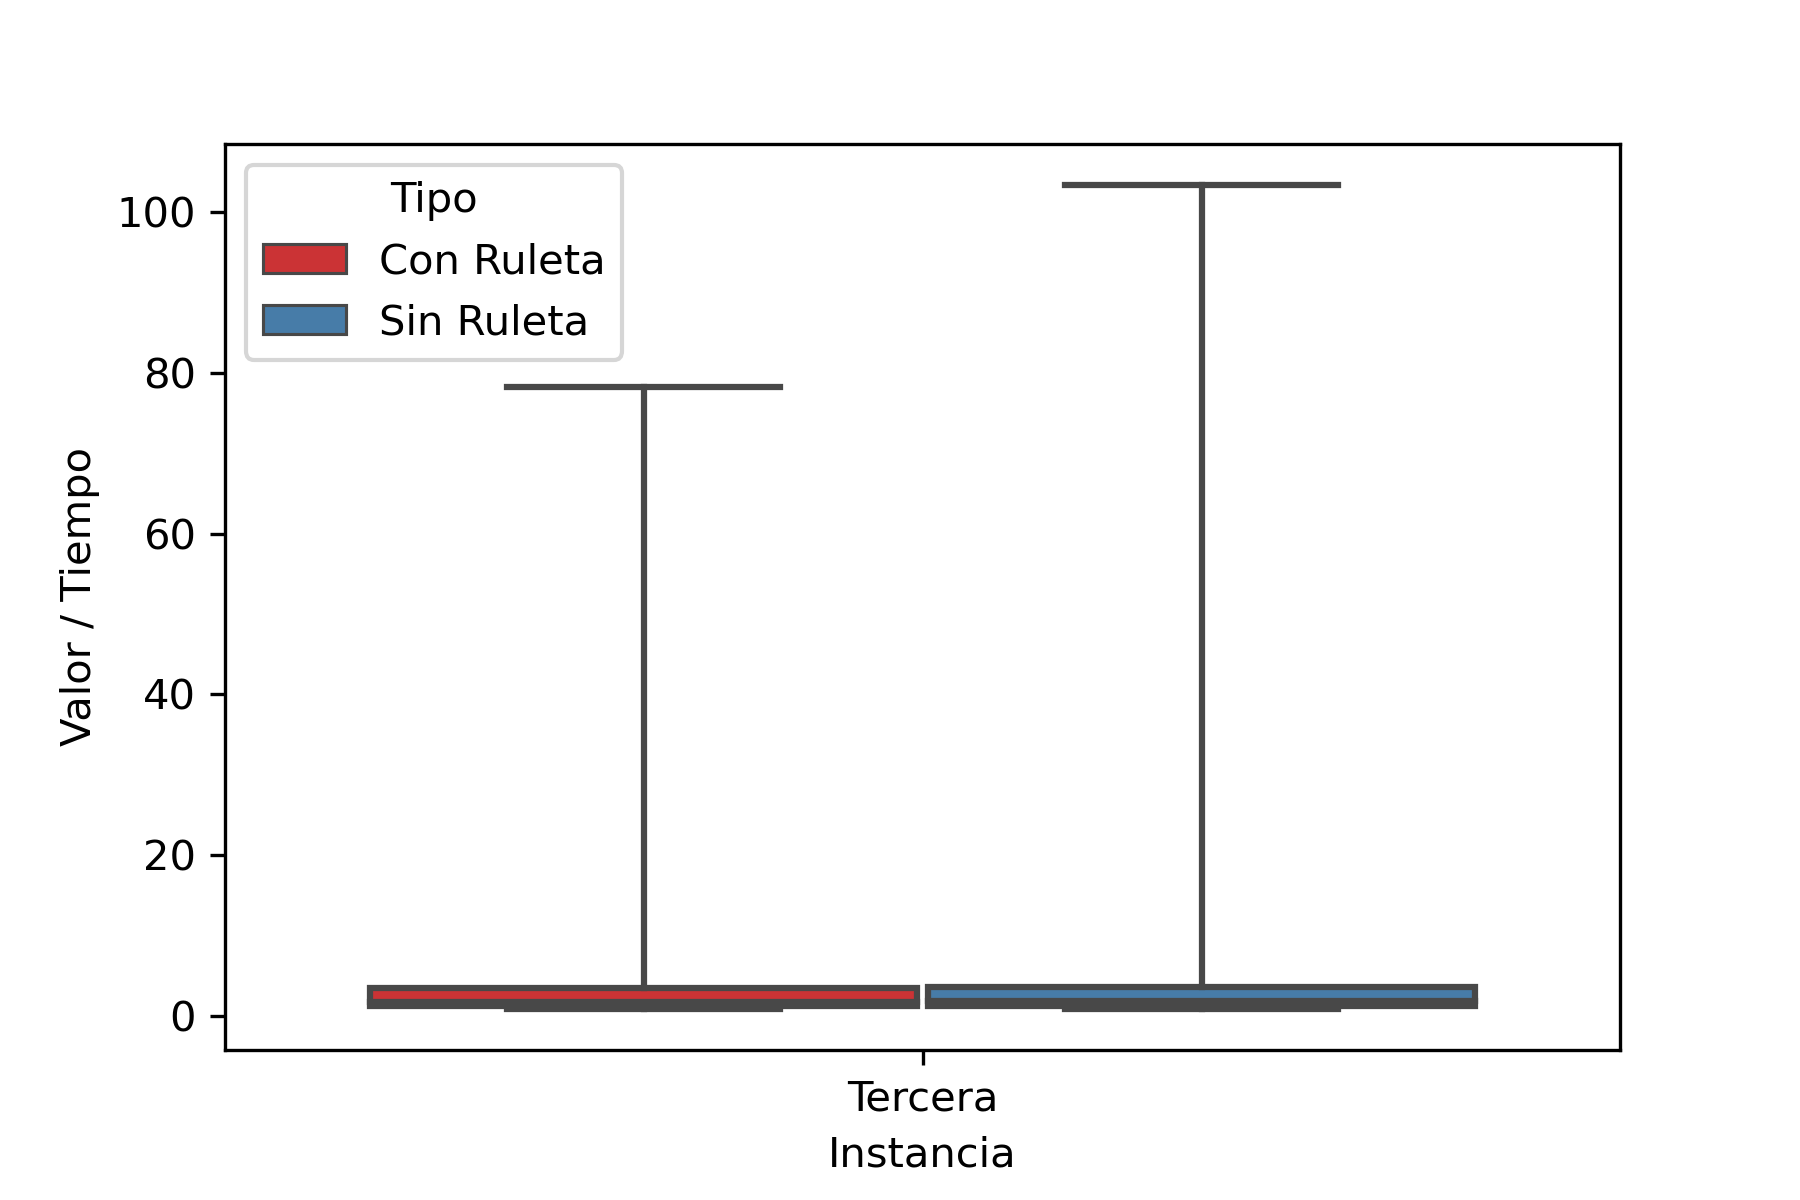
\includegraphics[width=\linewidth]{p10p_Box_Ter_100.png}
\caption{Caja bigote de tercera instancia con 100 objetivos.}
\end{subfigure}
\begin{subfigure}[b]{0.40\linewidth}
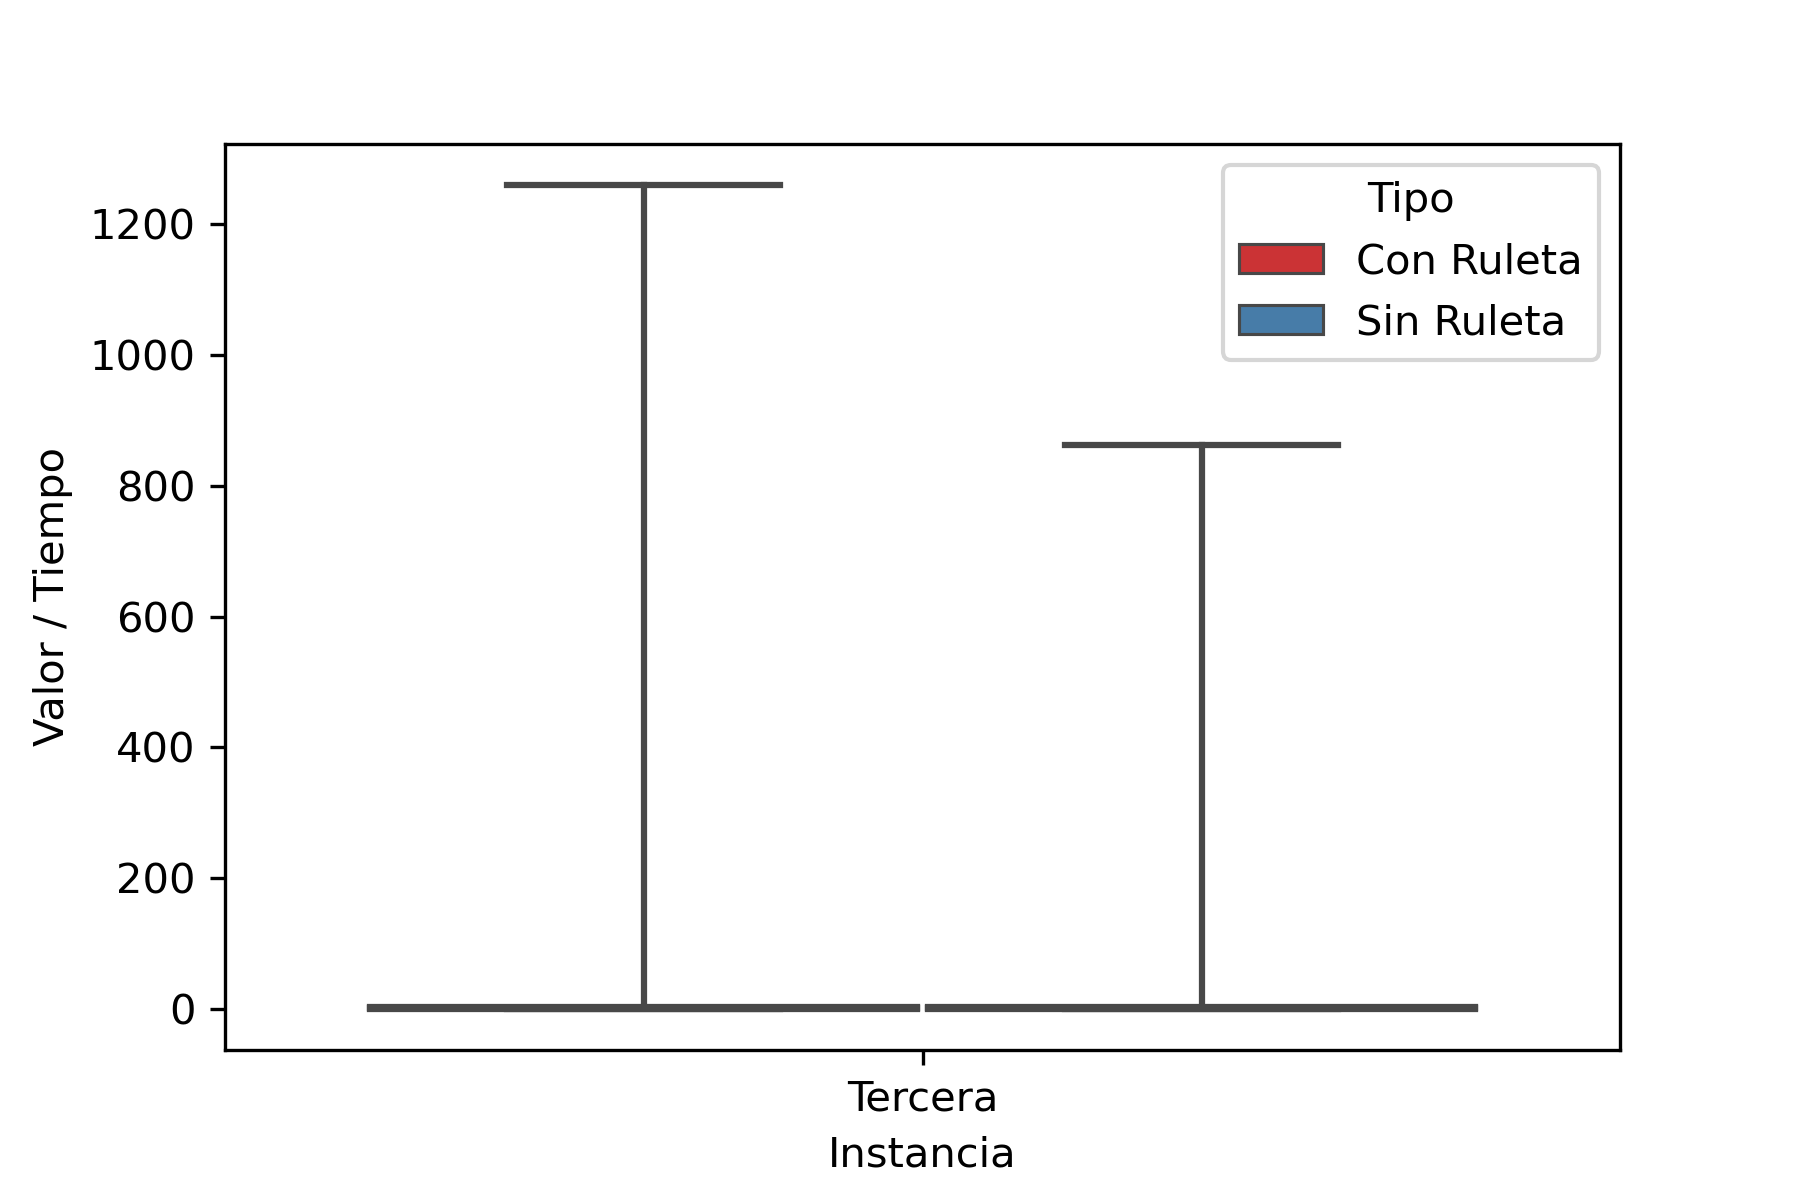
\includegraphics[width=\linewidth]{p10p_Box_Ter_400.png}
\caption{Caja bigote de tercera instancia con 400 objetivos.}
\end{subfigure}
\caption{Caja bigote comparando valor sobre tiempo para cada instancia.}
\label{fig:westminster}
\end{figure}

\begin{figure}[H]
\centering
\begin{subfigure}[b]{0.40\linewidth}
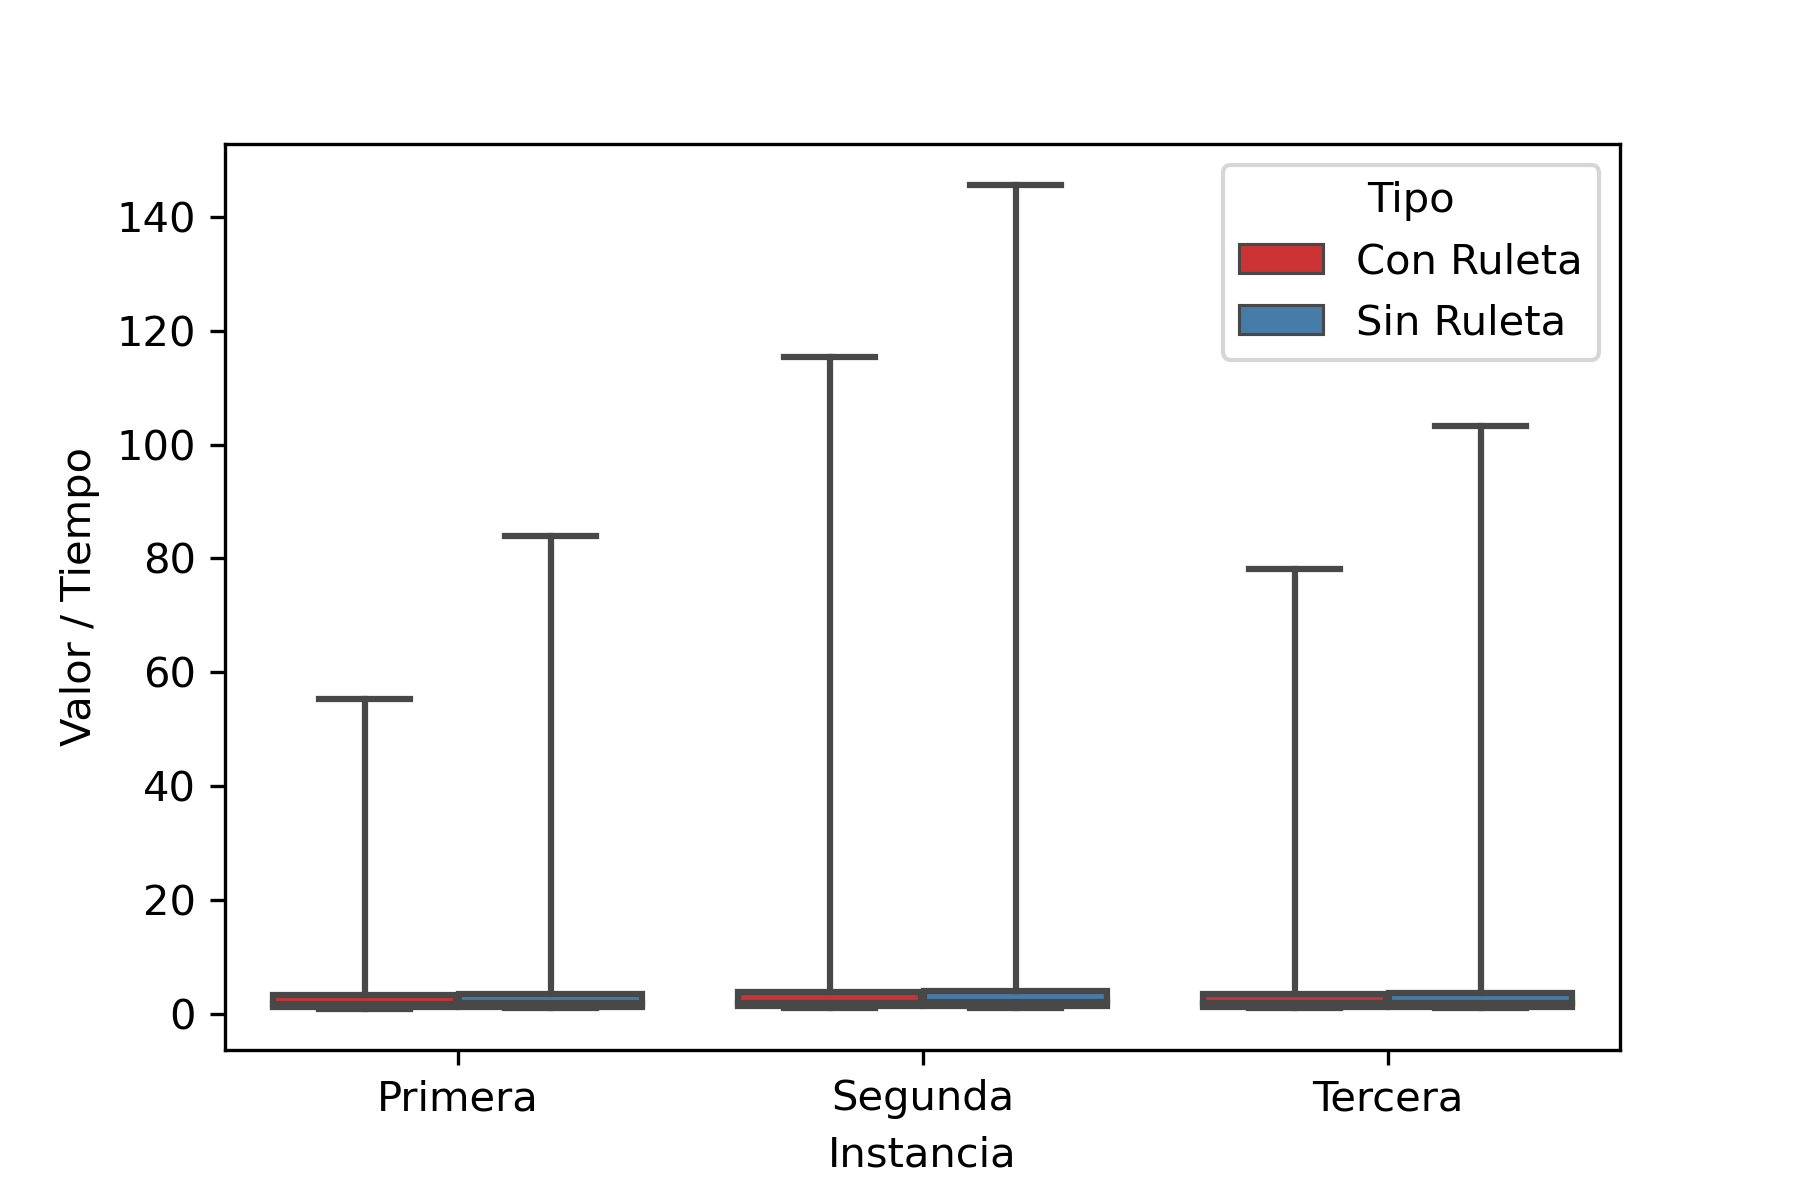
\includegraphics[width=\linewidth]{p10p_Box_Comp_100.png}
\caption{Caja bigote de las tres instancias con 100 objetivos.}
\end{subfigure}
\begin{subfigure}[b]{0.40\linewidth}
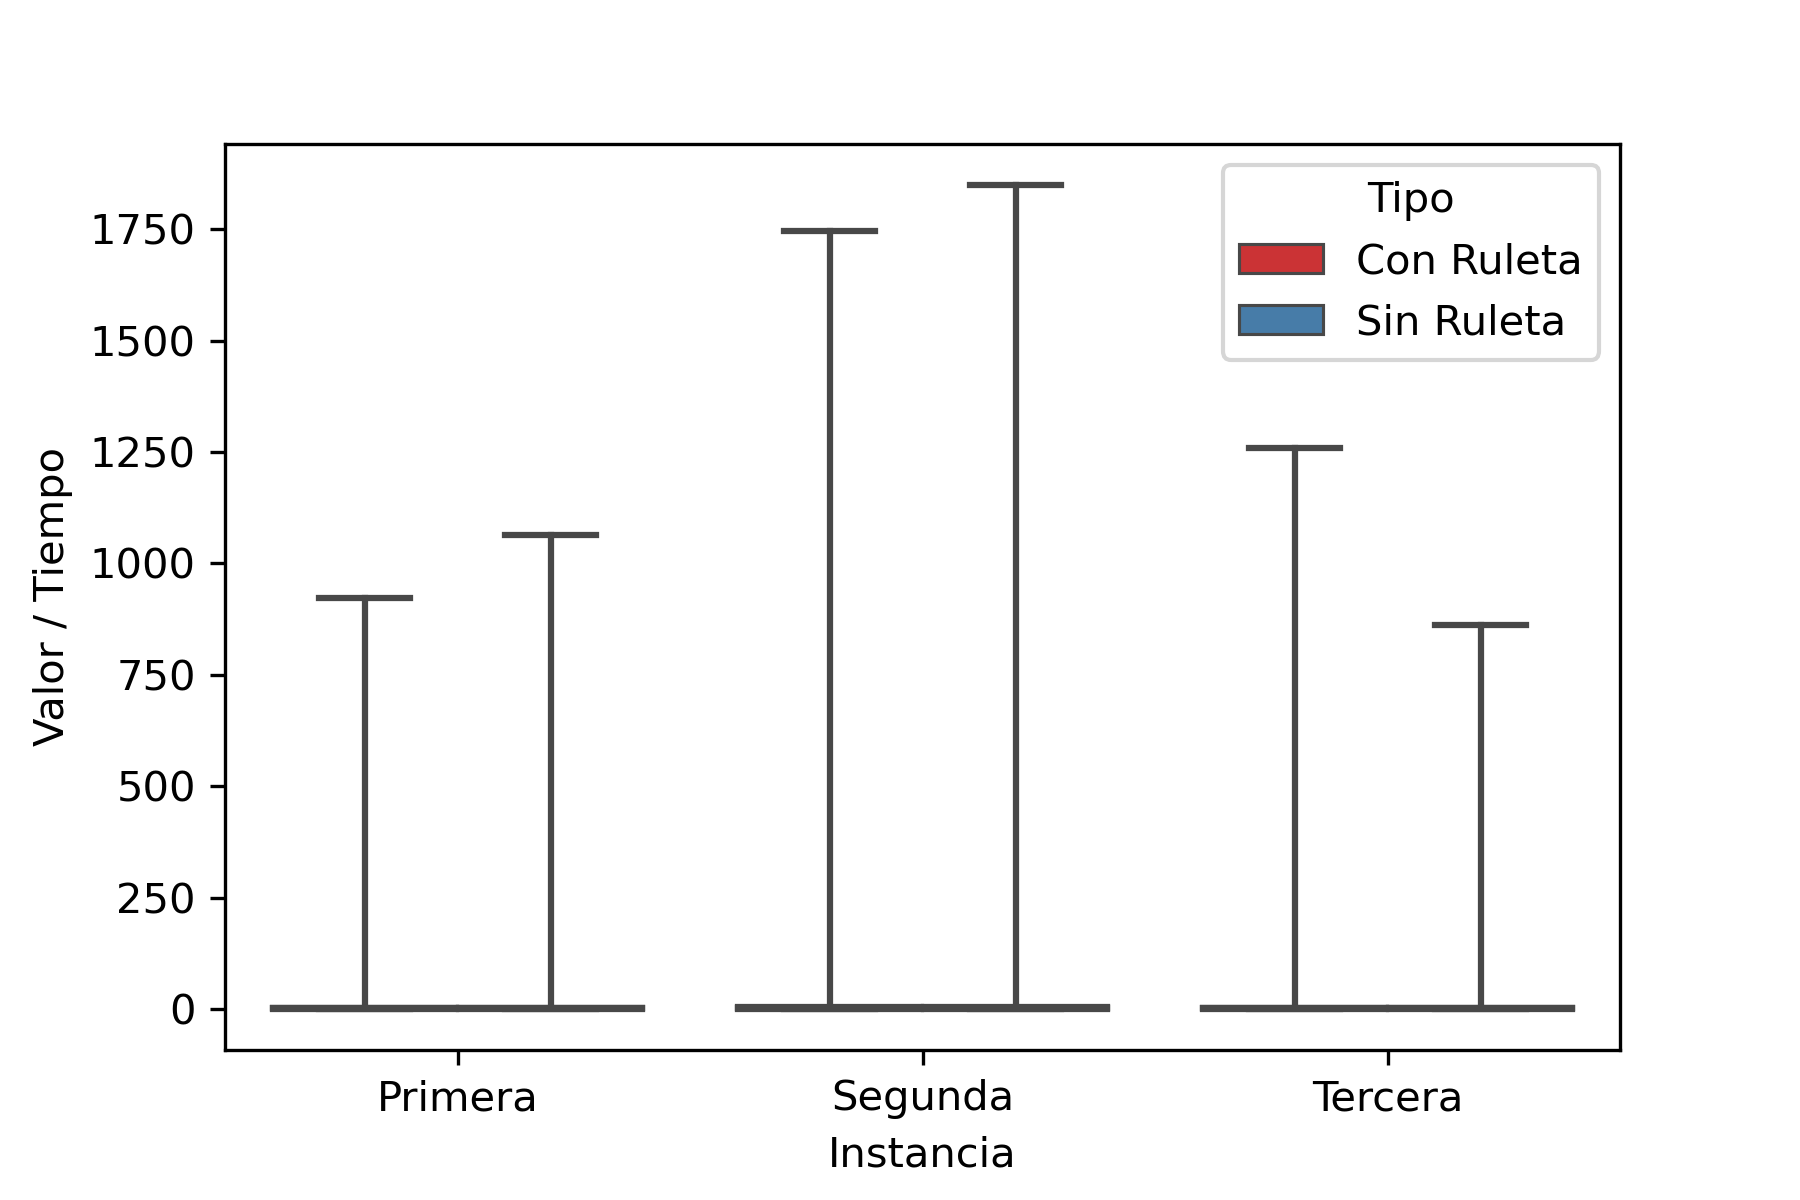
\includegraphics[width=\linewidth]{p10p_Box_Comp_400.png}
\caption{Caja bigote de las tres instancias con 400 objetivos.}
\end{subfigure}
\caption{Caja bigote comparando valor sobre tiempo para cada instancia.}
\label{fig:westminster}
\end{figure}

\section{Reto 1}
El primer reto es extender la selección de ruleta a la fase de supervivencia: en vez de quedarnos con las mejores soluciones, cada solución tiene una probablidad de entrar a la siguiente generación que es proporcional a su valor de la función objetivo, incorporando el sí o no es factible la solución en cuestión, permitiendo que los  mejores entre las factibles entren siempre (donde $k$ es un parámetro). Estudia nuevamente el efecto de este cambio en la calidad de la solución en los tres casos \cite{Satu_Elisa_Schaeffer}.
El código base se sacó de Schaeffer \cite{Elisa_Schaeffer}. El código completo se encuentra en el GitHub \cite{Denisse_Leyva}.

\renewcommand{\listingscaption}{Código}
\begin{listing}[H]
  \begin{minted}[linenos,mathescape,texcl]{clojure}
d = []
k = int(init * 0.1) # porcentaje que siempre entra
#Usamos el acomodo para obtener el 10% mejor que son 
#los que siempre van a entrar
for i in range(tam):
    d.append({'idx': i, 'obj': objetivo(p[i], valores),
              'fact': factible(p[i], pesos, capacidad)})
d = pd.DataFrame(d).sort_values(by = ['fact', 'obj'], ascending = False)
mantener = np.array(d.idx[:k])
popula = []
pesos_n = []
#Acomodamos los parametros para la Ruleta
for i in range(k, tam):
    vn = d.iloc[i]
    man = vn.idx
    o = vn.obj
    f = vn.fact
    popula.append(man)
    pesos_n.append((f+1)*o)
#Ruleta de suérvivencia
mantener2 = choices(population=popula, weights=pesos_n, k=(init-k))
#Guardamos valores de la ruleta
p2 = p[mantener2, :]
#Guardamos valores que siempre entran
p = p[mantener, :]
#Juntamos ambos arrays para tener el tamaño inicial
p = np.concatenate((p, p2), axis=0)
tam = p.shape[0]
      \end{minted}
  \label{lst:fibo}
  \caption{Genera la ruleta para la supervivencia.}
\end{listing}

\begin{figure}[H]
\centering
\begin{subfigure}[b]{0.40\linewidth}
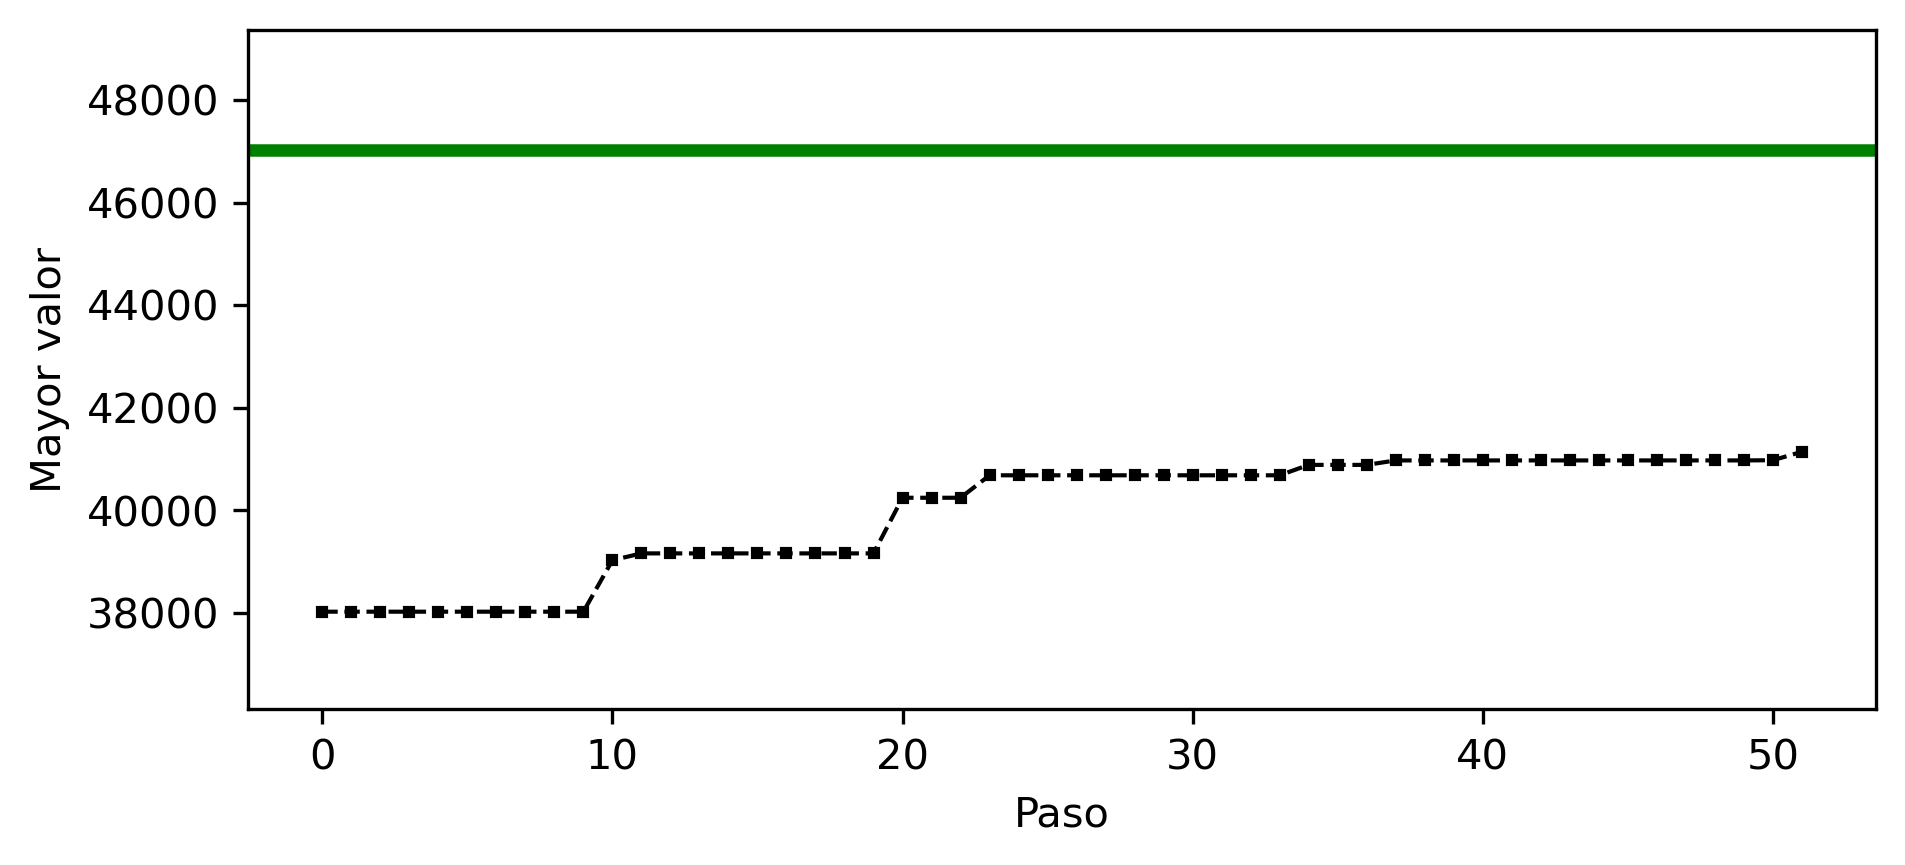
\includegraphics[width=\linewidth]{p10e_R_Prim_200R1.png}
\caption{Gráfica de primera instancia con ruleta a 200 objetivos.}
\end{subfigure}
\begin{subfigure}[b]{0.40\linewidth}
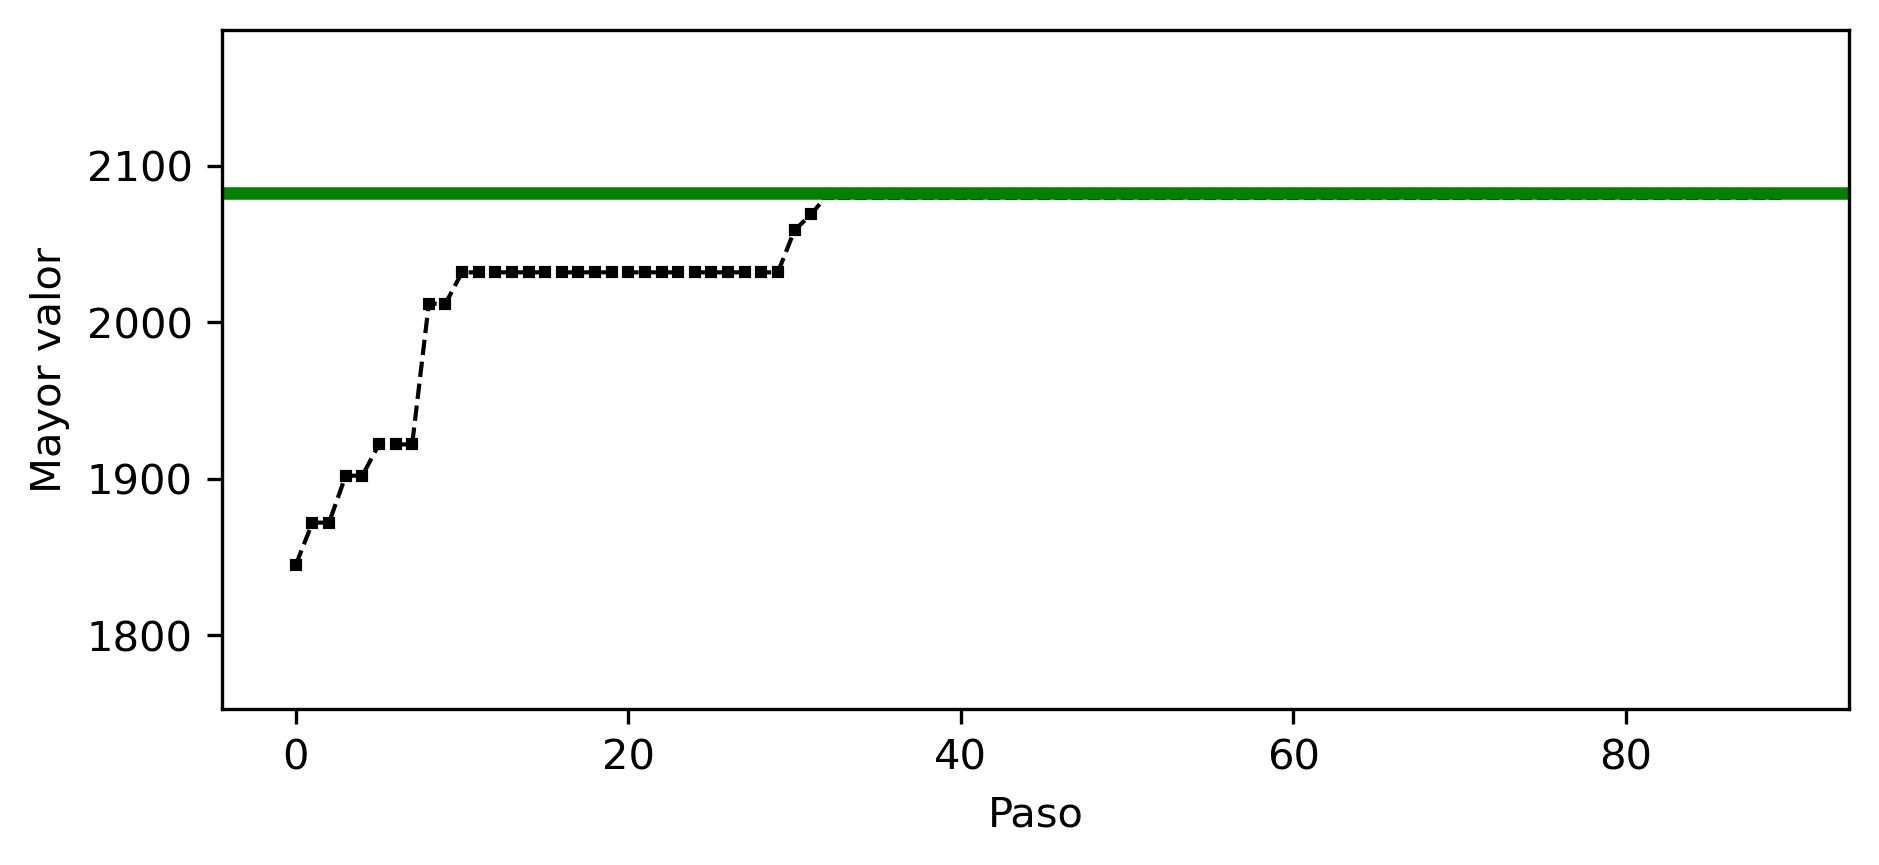
\includegraphics[width=\linewidth]{p10e_R_Seg_200R1.png}
\caption{Gráfica de segunda instancia con ruleta a 200 objetivos.}
\end{subfigure}
\caption{Gráficas comparando el mayor valor.}
\label{fig:westminster}
\end{figure}

\begin{figure}[H]
\centering
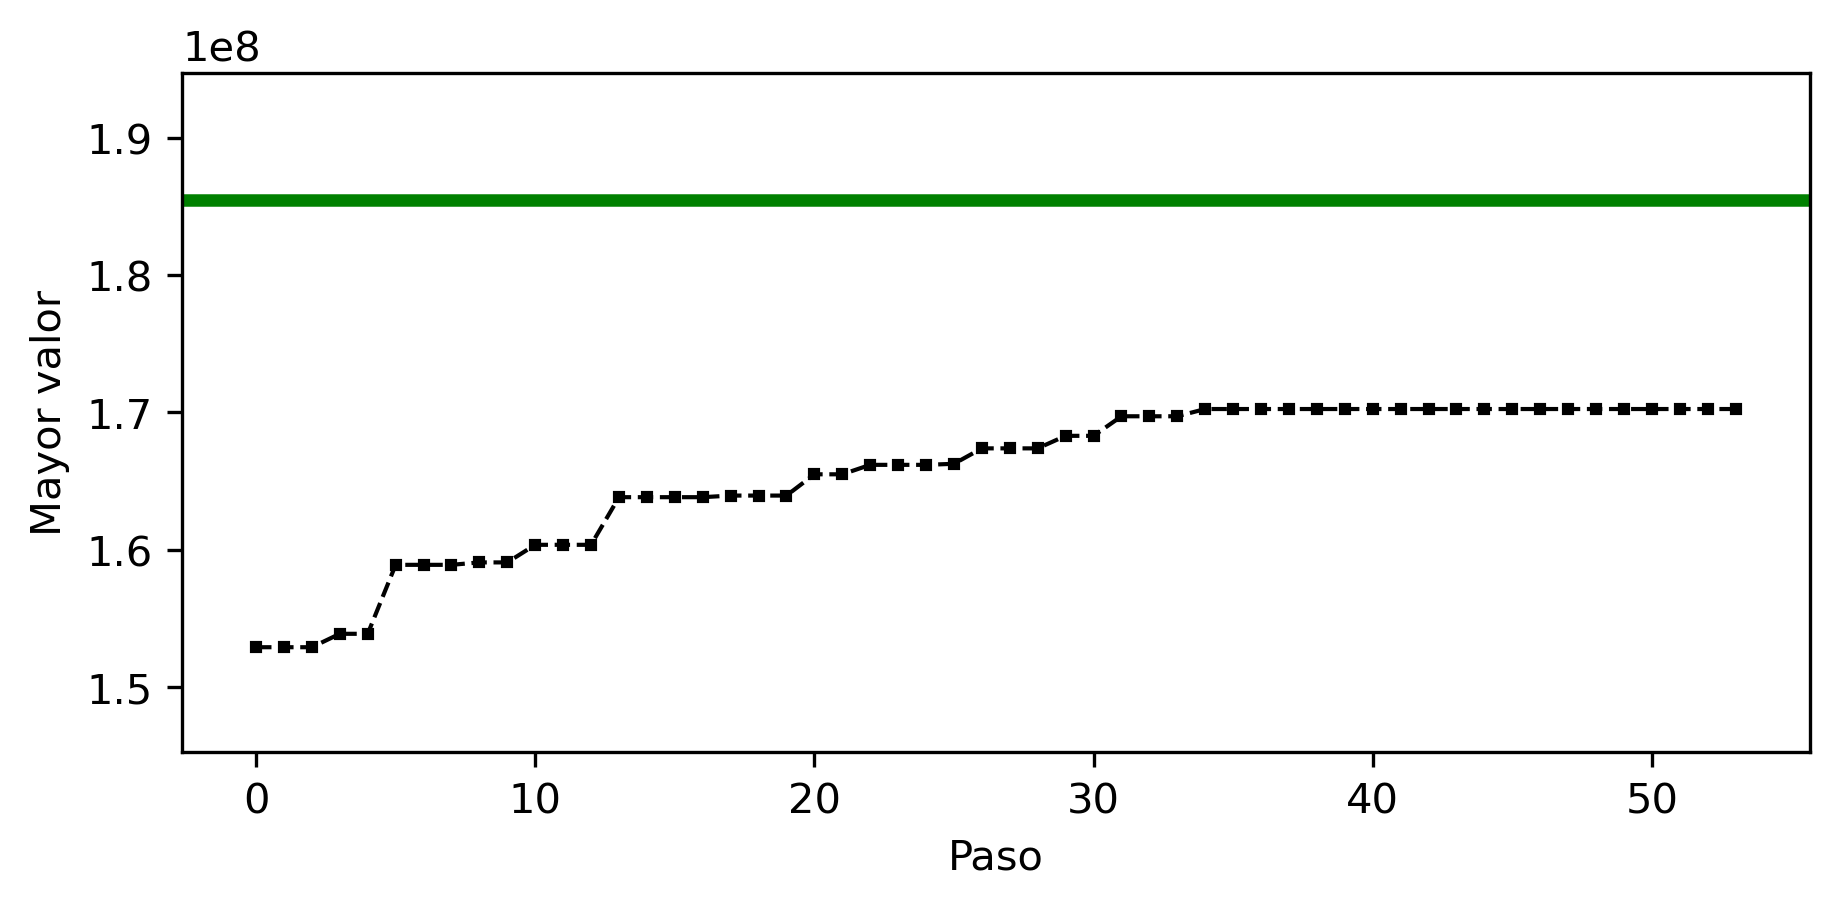
\includegraphics[width=80mm]{p10e_R_Ter_200R1.png}
\caption{\label{fig3} Gráfica de tercer instancia con ruleta a 200 objetivos.}
\end{figure}

\begin{figure}[H]
\centering
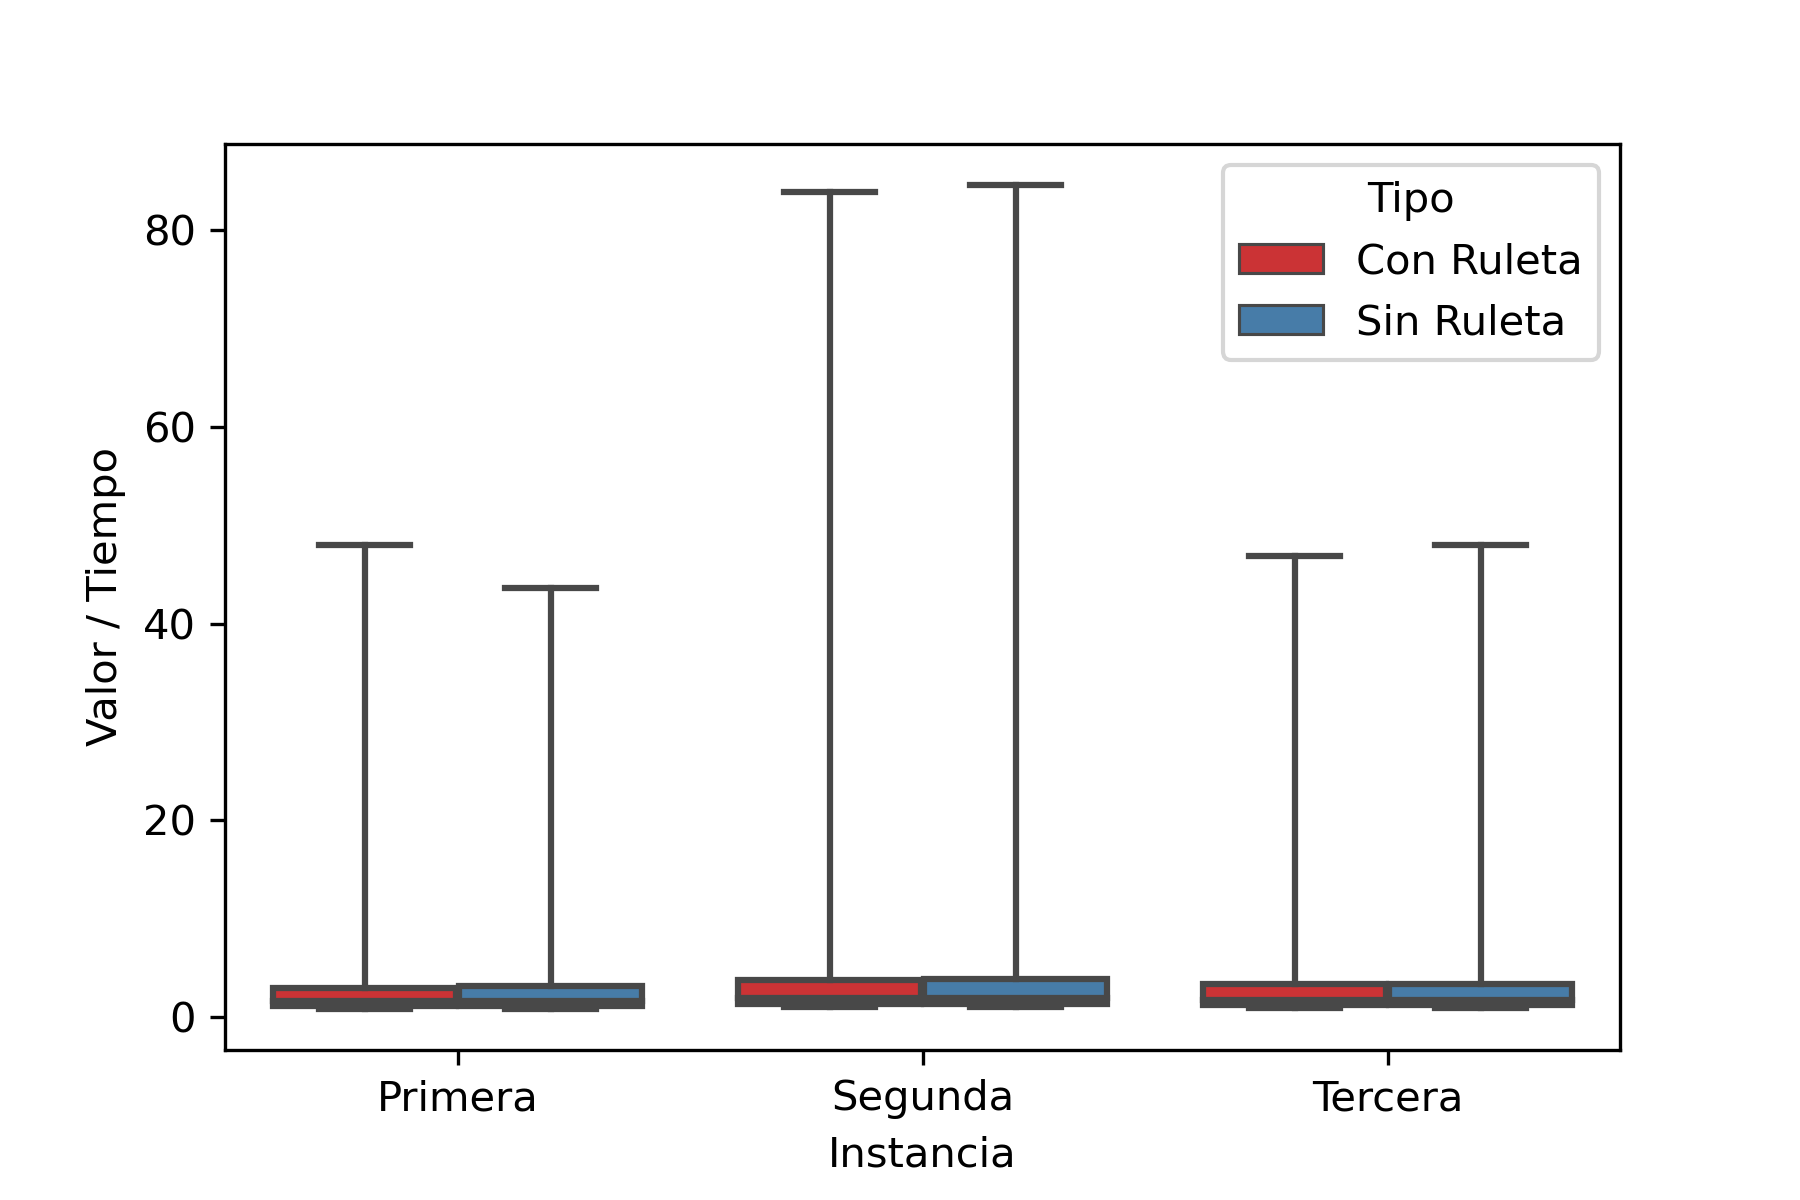
\includegraphics[width=80mm]{p10p_Box_Comp_200R1.png}
\caption{\label{fig3} Caja bigote de las tres instancias con 200 objetivos.}
\end{figure}

\begin{figure}[H]
\centering
\begin{subfigure}[b]{0.40\linewidth}
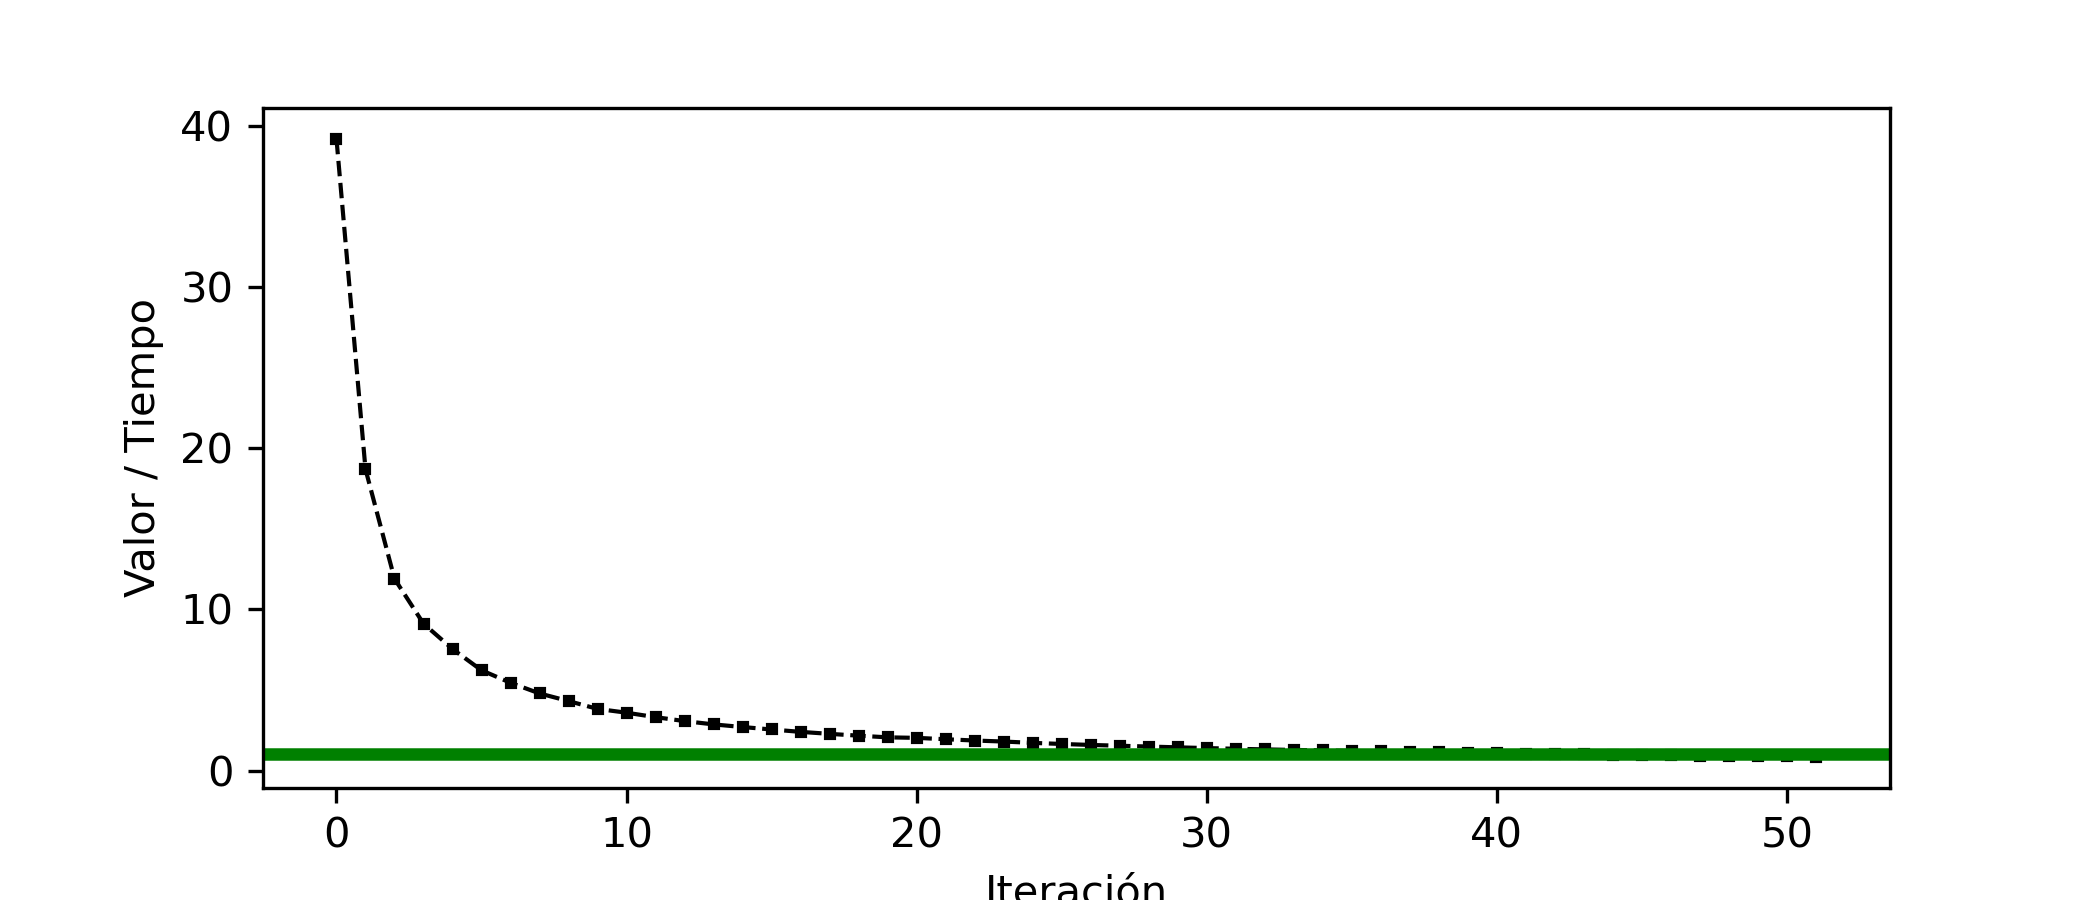
\includegraphics[width=\linewidth]{p10p_R_Prim_200R1.png}
\caption{Gráfica de primera instancia con ruleta a 200 objetivos.}
\end{subfigure}
\begin{subfigure}[b]{0.40\linewidth}
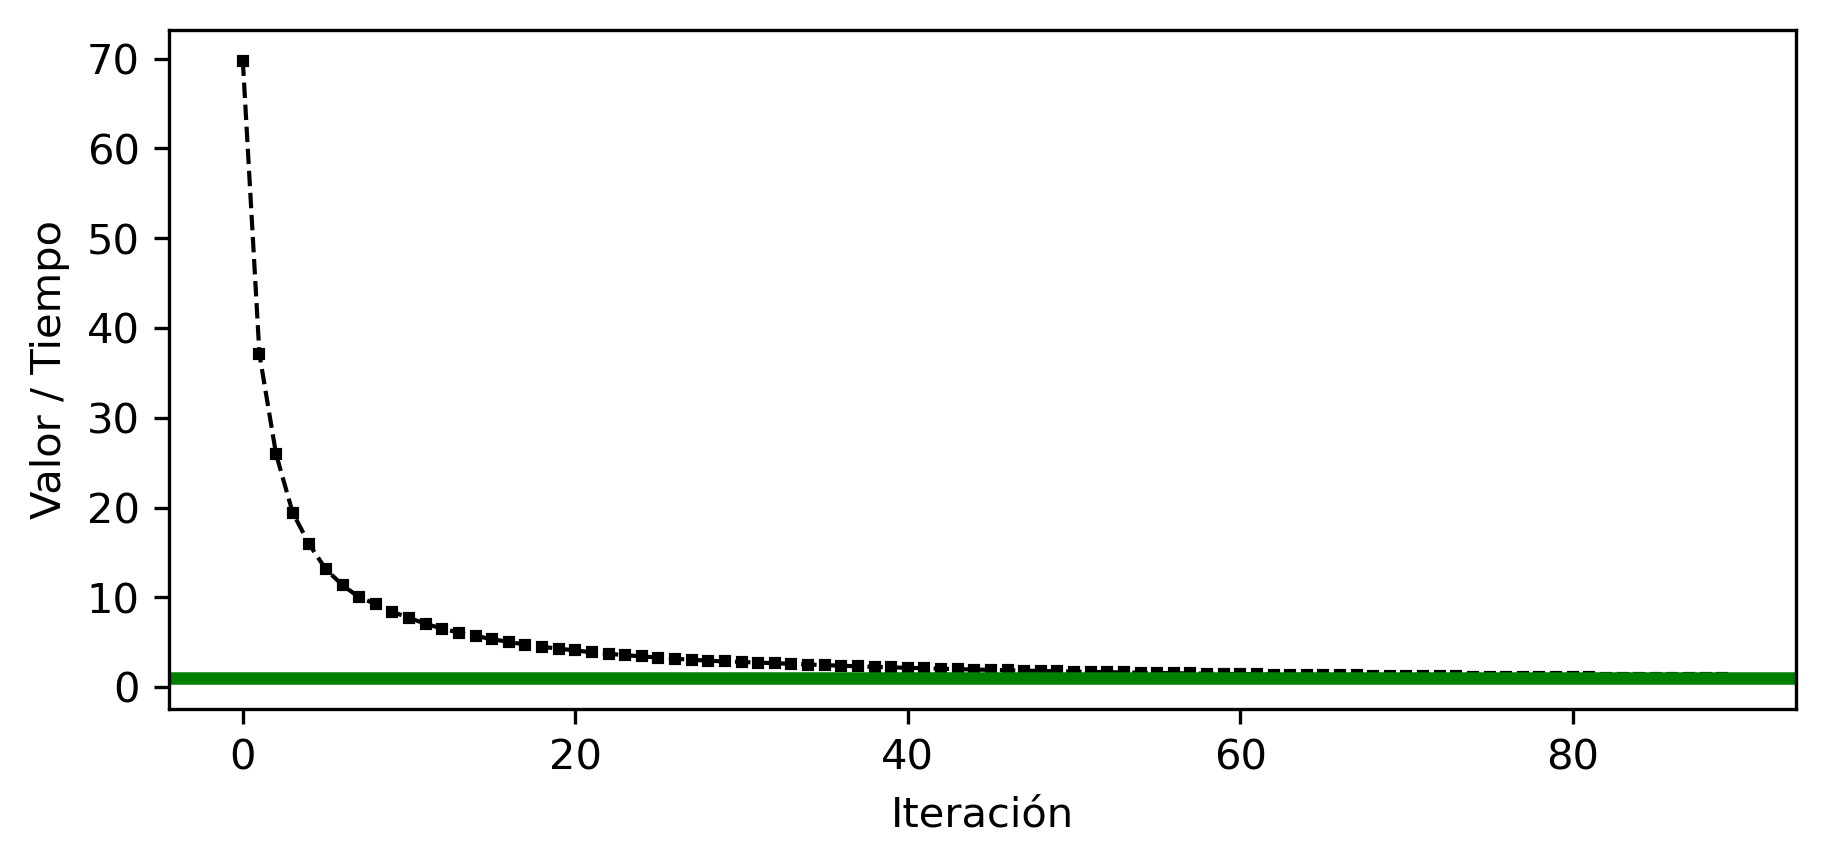
\includegraphics[width=\linewidth]{p10p_R_Seg_200R1.png}
\caption{Gráfica de segunda instancia con ruleta a 200 objetivoss.}
\end{subfigure}
\caption{Gráfica comparando valor sobre tiempo.}
\label{fig:westminster}
\end{figure}

\begin{figure}[H]
\centering
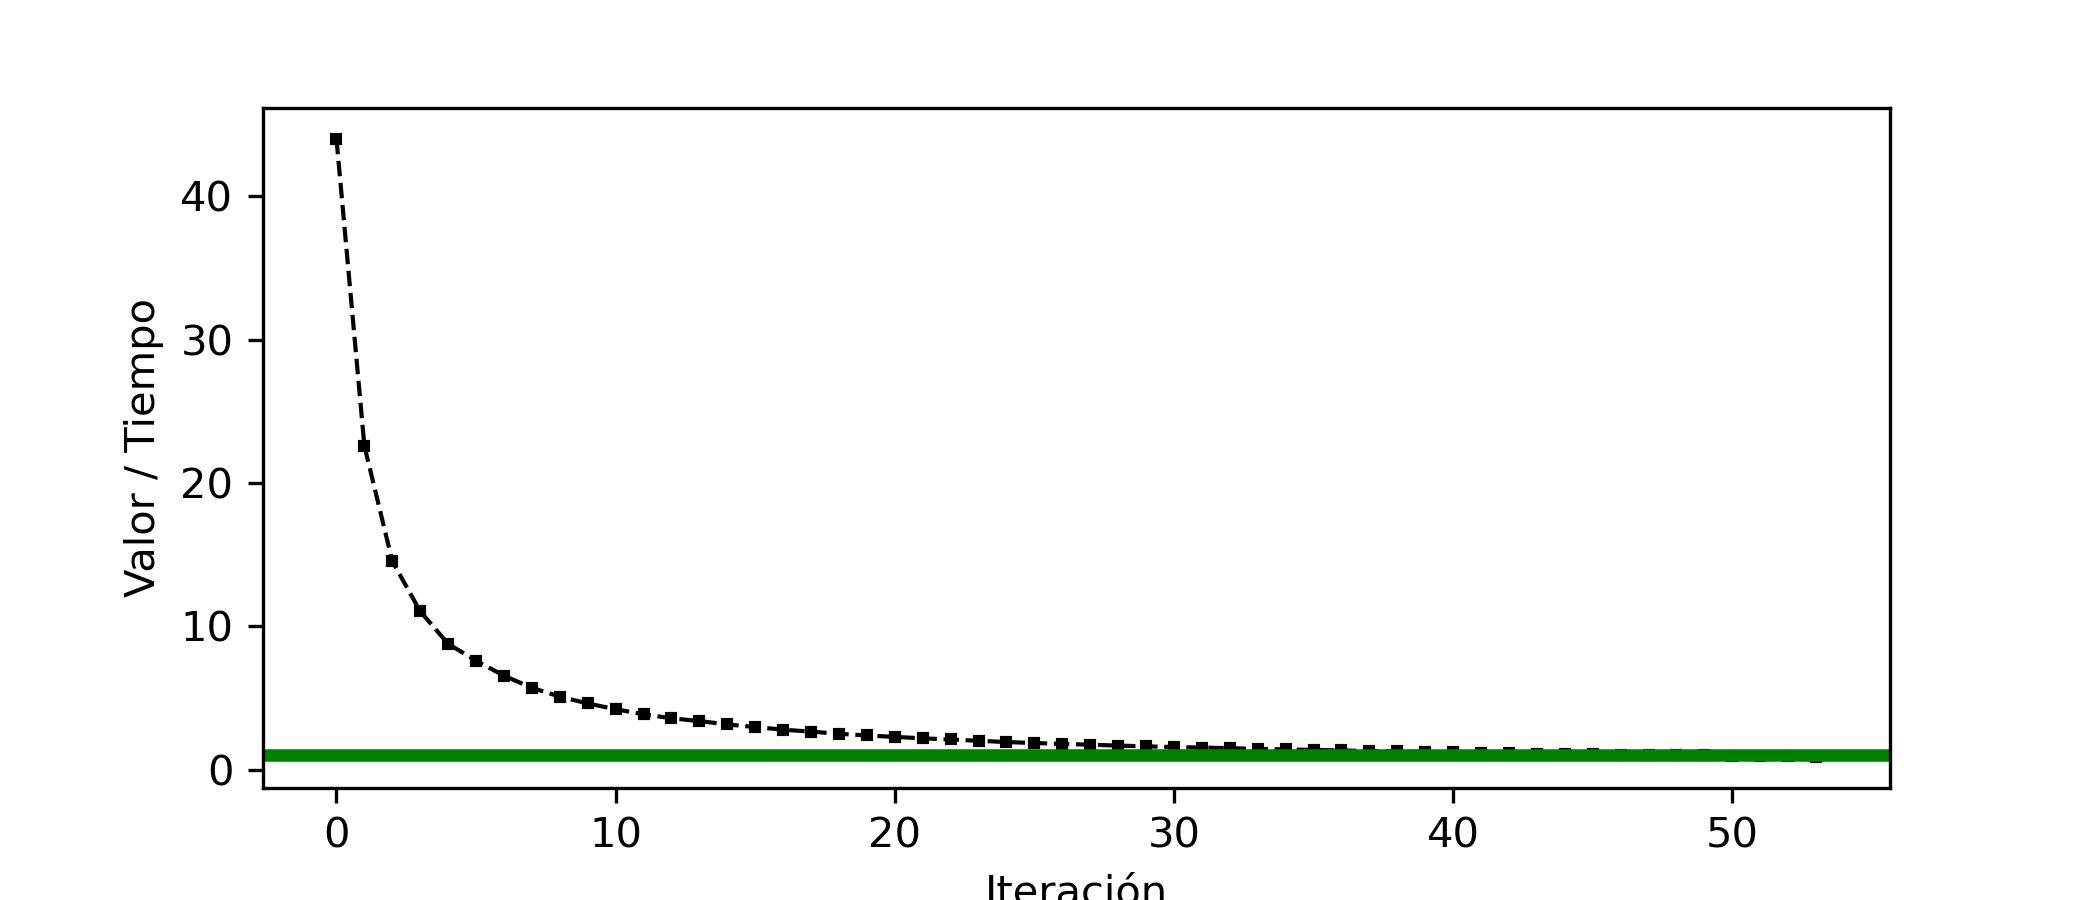
\includegraphics[width=80mm]{p10p_R_Ter_200R1.png}
\caption{\label{fig3} Gráfica de tercer instancia con ruleta a 200 objetivos.}
\end{figure}

\printbibliography
\end{document}
